\chapter{Results}
\label{sec:results}

This chapter first reports how the tool itself was checked, then the live evaluation
on fifteen prompts, the timing and area estimate, and live runs that show the trust
features at work. The older live runs from the first version of the system follow;
they are kept because they are still true records of what happened.

\section{Verification of the Tool}
\label{sec:verifymatrix}
\begin{table}[H]
\centering
\caption{Final verification status on the development machine (macOS, 19 November 2026).}
\label{tab:verify}
\footnotesize
\begin{tabularx}{\textwidth}{@{}p{3.0cm}p{4.9cm}X l@{}}
\toprule
\textbf{Check} & \textbf{Command} & \textbf{Result} & \textbf{Status} \\
\midrule
Backend suite & \code{python3 -m pytest} & 591 passed (35 files) & \textcolor{passgreen}{\textbf{PASS}} \\
Frontend unit tests & \code{npx vitest run} & 267 passed (18 files) & \textcolor{passgreen}{\textbf{PASS}} \\
TypeScript and build & \code{npx tsc -b}, \code{npm run build} & 0 errors; build succeeds & \textcolor{passgreen}{\textbf{PASS}} \\
Mutation sweep & \code{python3 tools/mutation_sweep.py} & 27 of 27 injected bugs caught & \textcolor{passgreen}{\textbf{PASS}} \\
Gate-level mapping & \code{python3 tools/verify_mapping.py} & 19 of 19 designs give the same results in gate-level simulation & \textcolor{passgreen}{\textbf{PASS}} \\
Formal equivalence & \code{equivalence.py} in the timing stage & 16 of 18 designs proven; 2 not proven (FSM state re-encoded); 0 different & see Table~\ref{tab:equiv} \\
Independent references & \code{python3 evaluation/independent/run.py} & 14 of 14 evaluated designs correct & \textcolor{passgreen}{\textbf{PASS}} \\
Accessibility & automated axe-core audit & 0 violations (both themes, passing and failing runs, every tab) & \textcolor{passgreen}{\textbf{PASS}} \\
Demo readiness & \code{python3 tools/preflight.py --live} & 0 failures, 0 warnings; all three fallback rungs ready & \textcolor{passgreen}{\textbf{PASS}} \\
Tools & \code{iverilog -V}, \code{yosys -V}, \code{sta -version} & Icarus 12.0, Yosys 0.71, OpenSTA 3.2.0 & available \\
\bottomrule
\end{tabularx}
\end{table}

The backend suite runs with Icarus, Yosys, OpenSTA and the sky130 library on
\code{PATH}, so no simulator or timing tests are skipped on this machine. The tests
that exercise the repair loop use real \code{iverilog}/\code{vvp} execution in
temporary workspaces. The newest components (separate testbench model, second
opinion, specification review, model menu) were also sabotaged on purpose, one
behaviour at a time, and the tests had to fail.

The independent reference testbenches (Section~\ref{sec:reftb}) check the evaluation
and not only the code. They were themselves measured with every one-token mutant the
generator can make (\code{evaluation/independent/strength.py}); every mutant they
missed is an equivalent change, unreachable code, or behaviour that the prompt does
not define.

\section{Live Evaluation on Fifteen Prompts}
\label{sec:eval}
Fifteen fixed prompts (7 combinational, 6 sequential, 2 FSM) were run through the
real pipeline with one free model, DeepSeek V4.1 Flash through the OpenCode app,
under the protocol of Section~\ref{sec:evalprotocol}. Table~\ref{tab:eval} gives the
results and Table~\ref{tab:evalprompts} the prompts.

\begin{table}[H]
\centering
\caption[Live evaluation on fourteen completed prompts]{Live evaluation, DeepSeek V4.1 Flash (free) through the OpenCode app. Strength = injected bugs caught / run. Toggle = measured toggle coverage of design signals. Timing = longest input-to-output path for designs with no clock, minimum clock period for clocked designs. Area is the pre-layout sky130 estimate.}
\label{tab:eval}
\footnotesize
\begin{tabular}{@{}l l l c r r r l r@{}}
\toprule
\textbf{ID} & \textbf{Type} & \textbf{Verdict} & \textbf{Repairs} & \textbf{Checks} & \textbf{Strength} & \textbf{Toggle} & \textbf{Timing} & \textbf{Area (\textmu m$^2$)} \\
\midrule
c1 & comb. & \textcolor{passgreen}{PASS} & 1 & 823/823 & 10/12 & 100\% & path 0.36 ns & 58.806 \\
c2 & comb. & \textcolor{passgreen}{PASS} & 1 & 308/308 & 1/1 & 100\% & path 0.12 ns & 26.275 \\
c3 & comb. & \textcolor{passgreen}{PASS} & 0 & 747/747 & 12/12 & 100\% & path 1.48 ns & 110.106 \\
c4 & comb. & \textcolor{passgreen}{PASS} & 0 & 907/907 & 6/6 & 100\% & path 0.63 ns & 205.197 \\
c5 & comb. & \textcolor{passgreen}{PASS} & 0 & 484/484 & 12/12 & 100\% & path 0.18 ns & 77.574 \\
c6 & comb. & \textcolor{passgreen}{PASS} & 1 & 2216/2216 & 3/3 & 100\% & path 0.44 ns & 95.091 \\
c7 & comb. & \textcolor{passgreen}{PASS} & 0 & 6909/6909 & 9/12 & 100\% & path 1.22 ns & 336.573 \\
s2 & seq. & \textcolor{passgreen}{PASS} & 0 & 2427/2427 & 9/9 & 100\% & min period 2.00 ns & 490.47 \\
s3 & seq. & \textcolor{passgreen}{PASS} & 0 & 2313/2313 & 5/5 & 100\% & min period 0.75 ns & 212.704 \\
s4 & seq. & \textcolor{passgreen}{PASS} & 1 & 2518/2518 & 3/3 & 100\% & min period 0.49 ns & 210.202 \\
s5 & seq. & \textcolor{passgreen}{PASS} & 0 & 275/275 & 7/7 & 100\% & min period 0.64 ns & 62.56 \\
s6 & seq. & \textcolor{passgreen}{PASS} & 0 & 2610/2610 & 12/12 & 100\% & min period 1.84 ns & 1830.51 \\
f1 & FSM & \textcolor{passgreen}{PASS} & 1 & 1287/1287 & 6/6 & 100\% & min period 0.74 ns & 163.907 \\
f2 & FSM & \textcolor{passgreen}{PASS} & 1 & 3797/3797 & 7/11 & 85\% & min period 1.25 ns & 466.698 \\
\midrule
s1 & seq. & \multicolumn{7}{l}{no result: testbench generation timed out three times (360 s, 600 s, 600 s)} \\
\bottomrule
\end{tabular}
\end{table}

\begin{table}[H]
\centering
\caption{The fifteen evaluation prompts (shortened).}
\label{tab:evalprompts}
\footnotesize
\begin{tabularx}{\textwidth}{@{}l X l X@{}}
\toprule
\textbf{ID} & \textbf{Prompt} & \textbf{ID} & \textbf{Prompt} \\
\midrule
c1 & 8-to-3 priority encoder with valid & s2 & 8-bit loadable up/down counter, synchronous reset \\
c2 & 4-bit binary to Gray code & s3 & 4-bit universal shift register \\
c3 & 4-bit ripple-carry adder & s4 & 8-bit SIPO shift register, synchronous reset \\
c4 & 4:1 multiplexer, 8-bit & s5 & clock divide-by-4, asynchronous reset \\
c5 & 3-to-8 decoder with enable & s6 & synchronous FIFO, 8-bit $\times$ 4, full/empty \\
c6 & 4-bit magnitude comparator & f1 & Moore 1011 detector (overlapping) \\
c7 & 4-bit ALU (add, sub, and, or, xor, overflow) & f2 & traffic light controller, synchronous reset \\
s1 & 4-bit up-counter (async reset, enable) & & \\
\bottomrule
\end{tabularx}
\end{table}

\paragraph{Summary.} Fourteen of the fifteen prompts completed, none through the
offline fallback. Eight passed on the first attempt, six passed after one self-repair
and none ended without a PASS. The median time per run was 360~s (3 to 13 minutes),
almost all of it model latency on the free tier. The strength score caught 102 of 111
injected bugs (92\%); eleven designs caught all of theirs, and the three that missed
some were c1 (10 of 12), c7 (9 of 12) and f2 (7 of 11). Toggle coverage was 100\%
except for f2 (85\%).

\paragraph{The missing prompt.} The fifteenth prompt, s1 (4-bit counter), did not
complete: testbench generation timed out on three separate attempts while the other
prompts finished. It is reported as ``no result'', never as a pass or as a design
failure. The same prompt passed on another free model
(\code{opencode/hy4-flash-free}, 173 of 173 checks), but that run used a different
model and is not counted in Table~\ref{tab:eval}.

\paragraph{Is a PASS here a correct design?} Each of the six repaired runs changed its
testbench during repair, which is the weakest kind of PASS. The strength score is
about the testbench, not the verdict, so every one of the 14 passing designs was also
run against the hand-written reference testbench described in
Section~\ref{sec:verifymatrix}. All 14 are correct: there was no false PASS in this
evaluation. The limits are that each prompt was run once, with one model, on small
blocks.

\section{Timing and Area Estimate}
\label{sec:timingres}
Table~\ref{tab:timing} gives the estimate for two built-in designs and the largest
evaluated design. A design with no clock is reported as its longest input-to-output
path, never as a clock rate. Figure~\ref{fig:timing} shows how the results panel
presents the estimate with its limits.

\begin{table}[H]
\centering
\caption{Pre-layout timing and area on \texttt{sky130\_fd\_sc\_hd} (typical corner, 25\,\textdegree C, 1.8\,V; no wire delay, ideal clock, setup only).}
\label{tab:timing}
\small
\begin{tabular}{@{}l r r l@{}}
\toprule
\textbf{Design} & \textbf{Cells} & \textbf{Area (\textmu m$^2$)} & \textbf{Timing} \\
\midrule
built-in 4-bit counter & 11 & 150.144 & min period 0.727 ns; meets 100 MHz with +9.27 ns slack \\
built-in 8-bit ALU & 109 & 636.861 & combinational: longest path 2.69 ns \\
FIFO (s6) & 120 & 1830.51 & min period 1.845 ns \\
\bottomrule
\end{tabular}
\end{table}

The numbers were checked, not assumed. \code{tools/verify_mapping.py} ran on 19
designs (the built-in designs and every saved evaluation design): for all 19, the
mapped gate netlist simulated with the same testbench gave the same pass counts as
the RTL; area and cell counts recomputed from the netlist and the liberty file matched
the reported values; and the implied minimum period did not change with the target
clock. The checker was also given sabotaged netlists and caught them. These checks
show that the estimate times the right circuit; it is still a pre-layout estimate, not sign-off.

\begin{figure}[htbp]
\centering
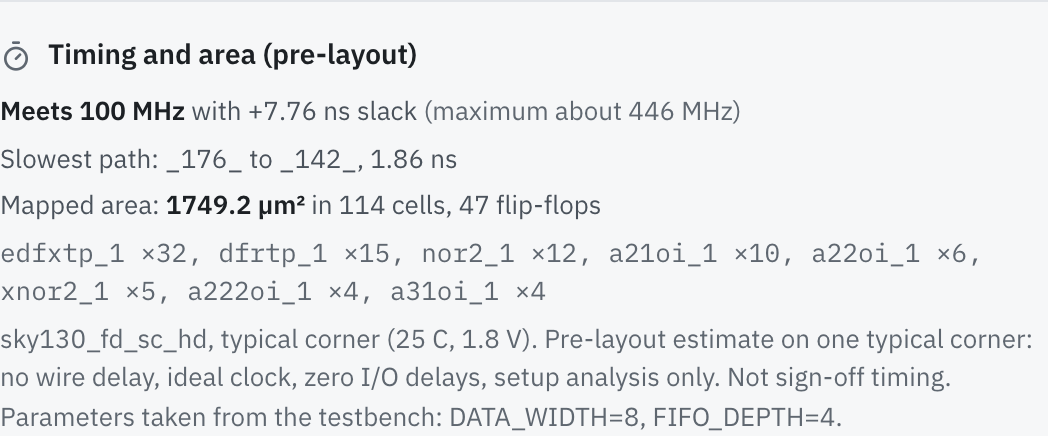
\includegraphics[width=0.65\textwidth]{s07_timing_section.png}
\caption[Timing and area section of the results panel]{Timing and area section of the results panel for a live FIFO run by \texttt{opencode/hy4-flash-free} (a different run from s6 in Table~\ref{tab:eval}): meets 100 MHz with +7.76 ns slack, 1749.2\,\textmu m$^2$ in 114 cells, with the limits of the estimate stated under the numbers and the testbench parameters that were applied.}
\label{fig:timing}
\end{figure}

\subsection{Formal equivalence and critical path}
\label{sec:equivres}
The formal check of Section~\ref{sec:equiv} was run on the 14 evaluation designs and
four built-in designs (the 4-bit counter, the 8-bit ALU, the adder and the 4:1 multiplexer). Table~\ref{tab:equiv} gives the result. All combinational and
sequential designs were formally proven equivalent (Yosys SAT). The two FSMs, f1 and
f2, were reported as ``not proven'': synthesis re-encoded their state, so the
registers could not be paired by name and induction could not decide. Both still pass
the gate-level simulation check. No design was reported as different. To see that the
check can fail, the netlist of the built-in 4-bit ALU was sabotaged on purpose (one
\code{nand2} cell replaced by a \code{nor2} cell, which has the same pins); the check
reported it as different. This sabotage case is an automated test.

\begin{table}[H]
\centering
\caption{Formal equivalence of the sky130 netlist and the RTL (19 November 2026).}
\label{tab:equiv}
\footnotesize
\begin{tabularx}{\textwidth}{@{}p{4.2cm}c l X@{}}
\toprule
\textbf{Designs} & \textbf{Count} & \textbf{Method} & \textbf{Result} \\
\midrule
Evaluation, combinational (c1--c7) & 7 & miter + SAT & 7 proven \\
Evaluation, sequential (s2--s6) & 5 & temporal induction & 5 proven \\
Evaluation, FSM (f1, f2) & 2 & temporal induction & 2 not proven (state re-encoded by synthesis) \\
Built-in (counter, 8-bit ALU, adder, mux) & 4 & SAT or induction & 4 proven \\
\midrule
\textbf{Total} & \textbf{18} & & \textbf{16 proven, 2 not proven, 0 different} \\
\midrule
Built-in 4-bit ALU, one \code{nand2} changed to \code{nor2} & 1 & miter + SAT & reported as different (sabotage check) \\
\bottomrule
\end{tabularx}
\end{table}

``Proven'' here means that the mapped netlist computes the same function as the RTL.
It does not mean that the RTL is correct; that is shown, as far as it can be, by the
testbench, the strength score and the reference testbenches of
Section~\ref{sec:eval}.

Figure~\ref{fig:critpath} shows the timing section of the built-in 8-bit ALU, which
has no clock. The longest input-to-output path is 2.69\,ns, from \code{b[0]} to
\code{overflow}. The critical path table explains why: after one \code{nor2b_1} cell
the path goes through six \code{maj3_1} cells, the ripple-carry chain of the adder,
at about 0.36 to 0.39\,ns each, then through \code{o21ai_0} and \code{o22ai_1} to the output.
A carry-lookahead or carry-select adder is the change that would shorten this path.

\begin{figure}[htbp]
\centering
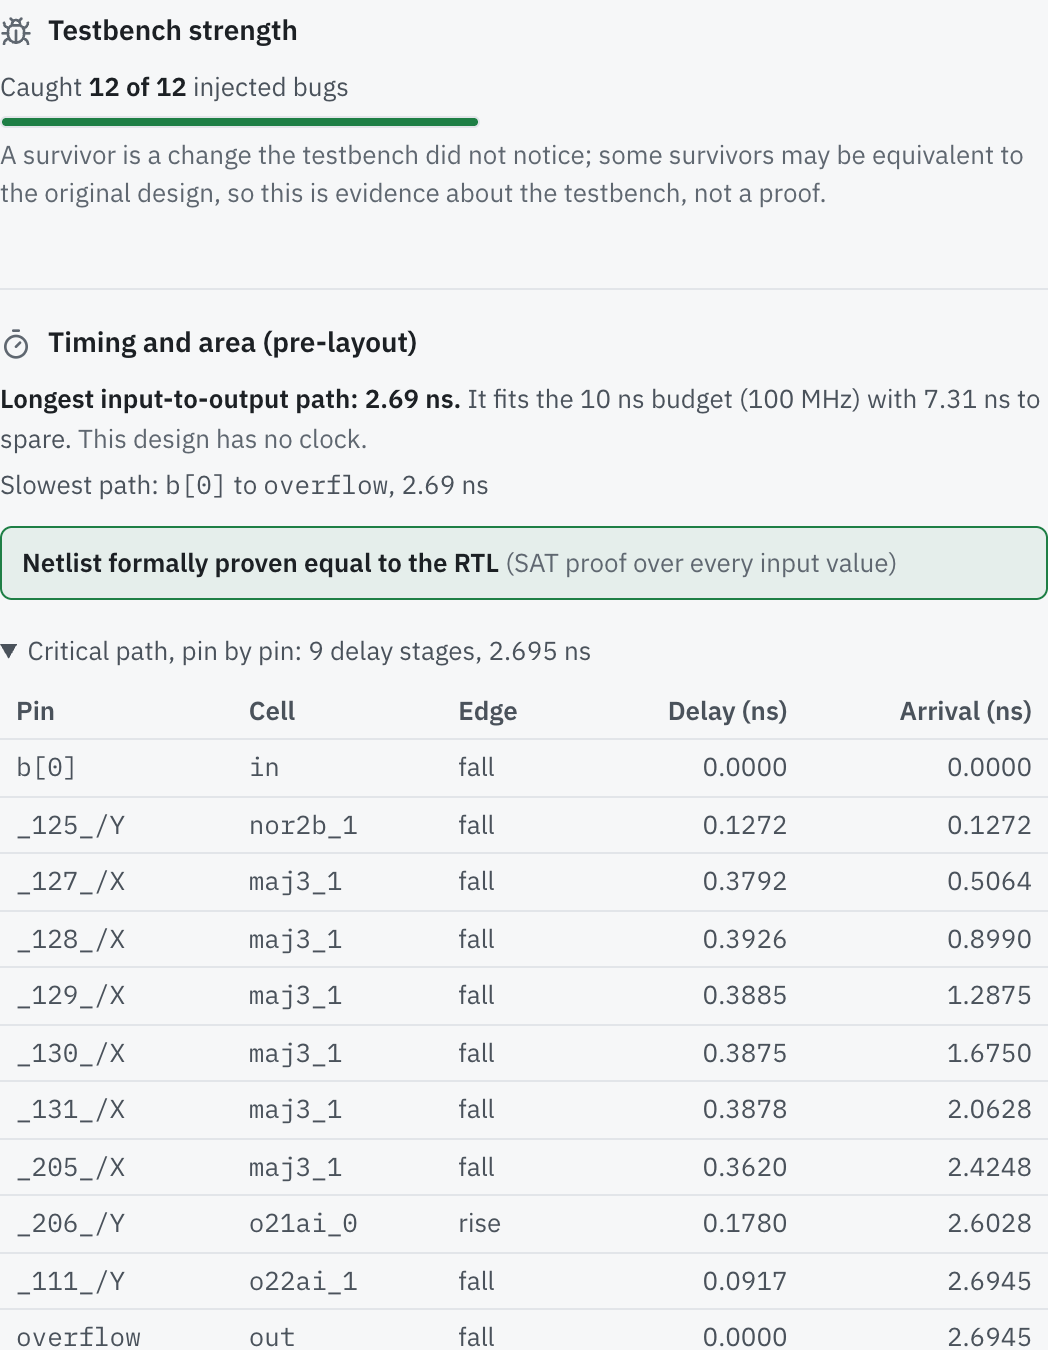
\includegraphics[width=0.45\textwidth]{s20_timing_proof_critical_path.png}
\caption[Timing section with the equivalence result and the critical path]{Results panel of the \emph{built-in} 8-bit ALU (offline demo design, not an AI result): longest path 2.69\,ns, the line ``Netlist formally proven equal to the RTL (SAT proof over every input value)'' and the critical path pin by pin, with the sky130 cell, edge, delay and arrival of each stage.}
\label{fig:critpath}
\end{figure}

\section{Trust Features in Live Runs}
\label{sec:trustres}

\subsection{Model menu and switching}
The model menu (Figure~\ref{fig:models}) was tested live. Three different free
OpenCode models answered a live probe in about 3~s each. The Cloudflare Workers AI
catalogue listed 40 text models and the NVIDIA NIM catalogue 15 chat models. The
fastest NIM chat models answered in about 1 to 7~s, but some free-queue models took 1
to 5 minutes for one reply. Two failures showed why catalogues are read live and never
hard-coded: DeepSeek V4.1 Flash on NIM was retired on 16 November 2026 (HTTP 410), and
GLM-5.3-flash and DeepSeek V4.1 Flash are refused on the Cloudflare Workers Free plan
(HTTP 403, code 5035). A chosen model that fails in such a way is reported in plain
words and is never replaced by the scripted demo.

\begin{figure}[htbp]
\centering
\begin{minipage}[t]{0.36\textwidth}
\vspace{0pt}\centering
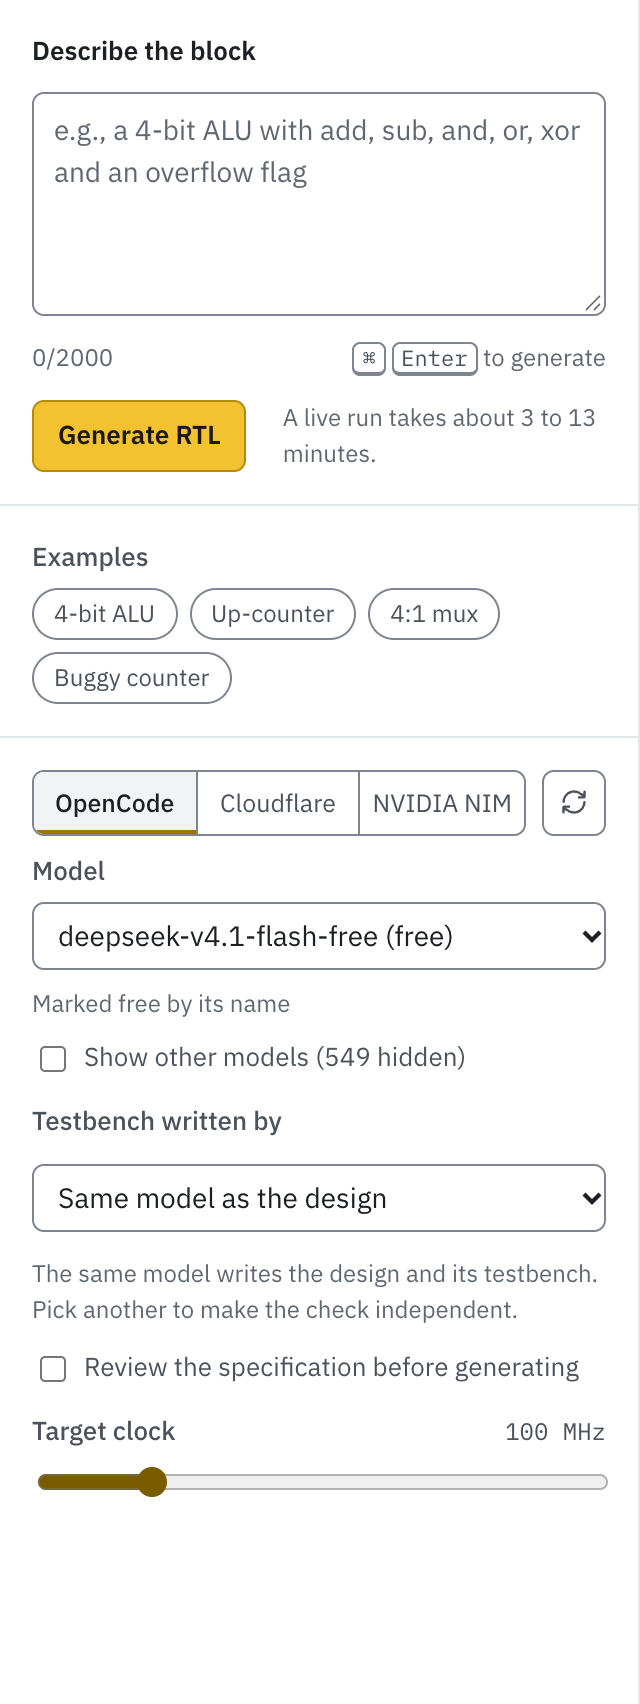
\includegraphics[height=8cm]{s02_model_menu.png}\par\small (a)
\end{minipage}\hspace{0.06\textwidth}
\begin{minipage}[t]{0.36\textwidth}
\vspace{0pt}\centering
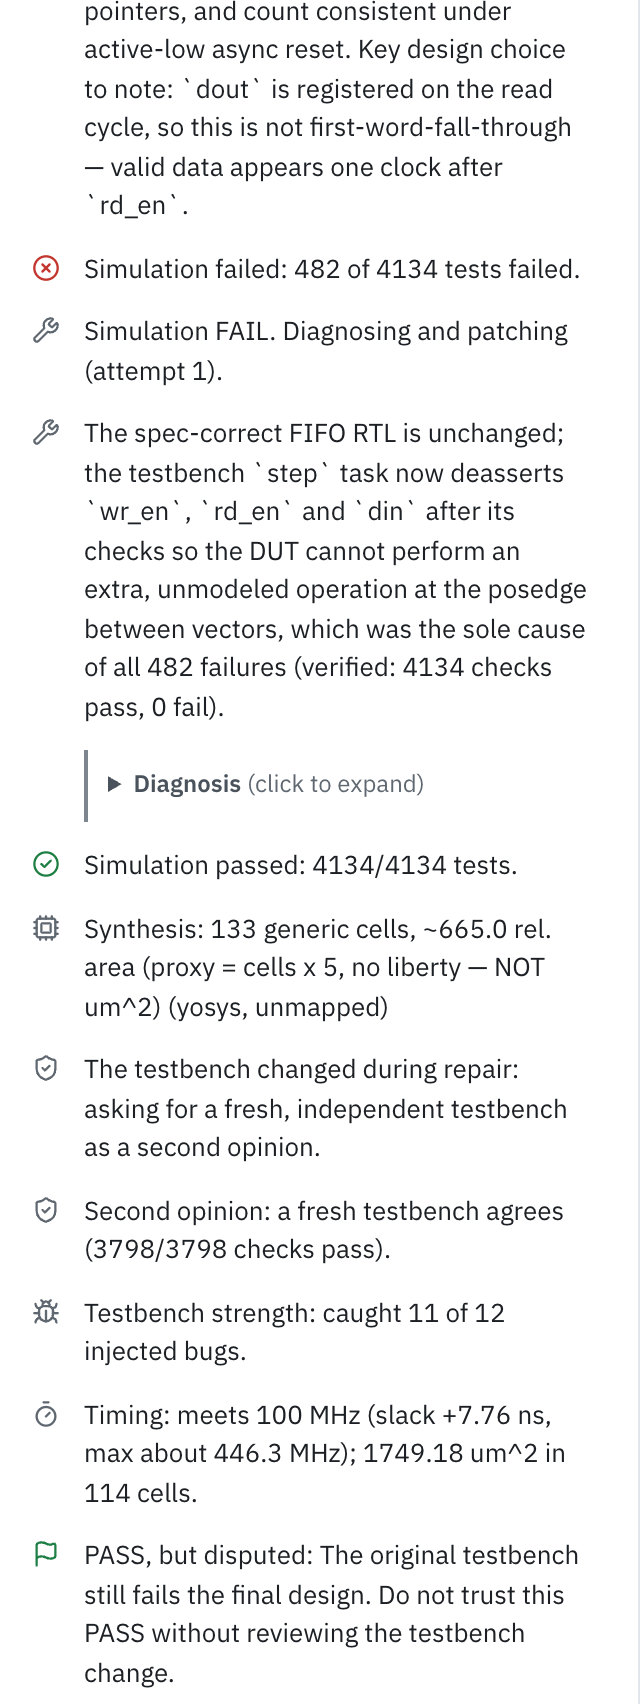
\includegraphics[height=8cm]{s05_run_timeline.png}\par\small (b)
\end{minipage}
\caption[Model menu and run timeline]{(a) The sidebar with the prompt box, the per-run Model menu (OpenCode, Cloudflare Workers AI, NVIDIA NIM), the ``Testbench written by'' choice, the specification-review option and the target clock. (b) End of the run timeline of the live FIFO run of Figure~\ref{fig:second}: the repair's explanation, the PASS, the second opinion, strength and timing messages.}
\label{fig:models}
\end{figure}

\subsection{Verdict integrity on another provider}
A full run on Cloudflare's \code{gpt-oss-120b} wrote a correct counter but a
testbench whose watchdog timer was shorter than its own test. The simulation ended
before the summary was printed, so the run was ERROR with 0 checks, and the
application refused to call it PASS. The verdict rules hold whichever model writes
the testbench.

\subsection{Separate testbench model}
With \code{opencode/hy4-flash-free} writing the design and
\code{nim/poolside/laguna-xs-2.1} writing the testbench, the 4-bit counter run ended
\textcolor{failred}{\textbf{FAIL}} with 124 of 146 checks passing. The counter was
correct; the testbench sampled the output one cycle early. Because the testbench came
from a separate model, the design model was not allowed to rewrite the failing checks
away, and the result stated that the two models disagree. The application does not
decide which side is wrong: a person compares the first failing check with the
specification, which is what showed the testbench error here.

A second run with the same two models, a 4-bit universal shift register, behaved the
same way (Figure~\ref{fig:indepfail}): \textcolor{failred}{\textbf{FAIL}} with 61 of
108 checks passing. The design model's diagnosis blamed the testbench and left the RTL
unchanged, and the application did not apply its testbench change, because a
separate model wrote the testbench. A check by hand afterwards found two reset
mistakes in the testbench (no reset edge at time zero, and reset never released before
its exhaustive section). Fixing only those two testbench lines gave 108 of 108 with
the unchanged RTL, so the design was correct. The model's diagnosis had named the
right side but not the real defects, which is why the decision is left to a person.

\begin{figure}[htbp]
\centering
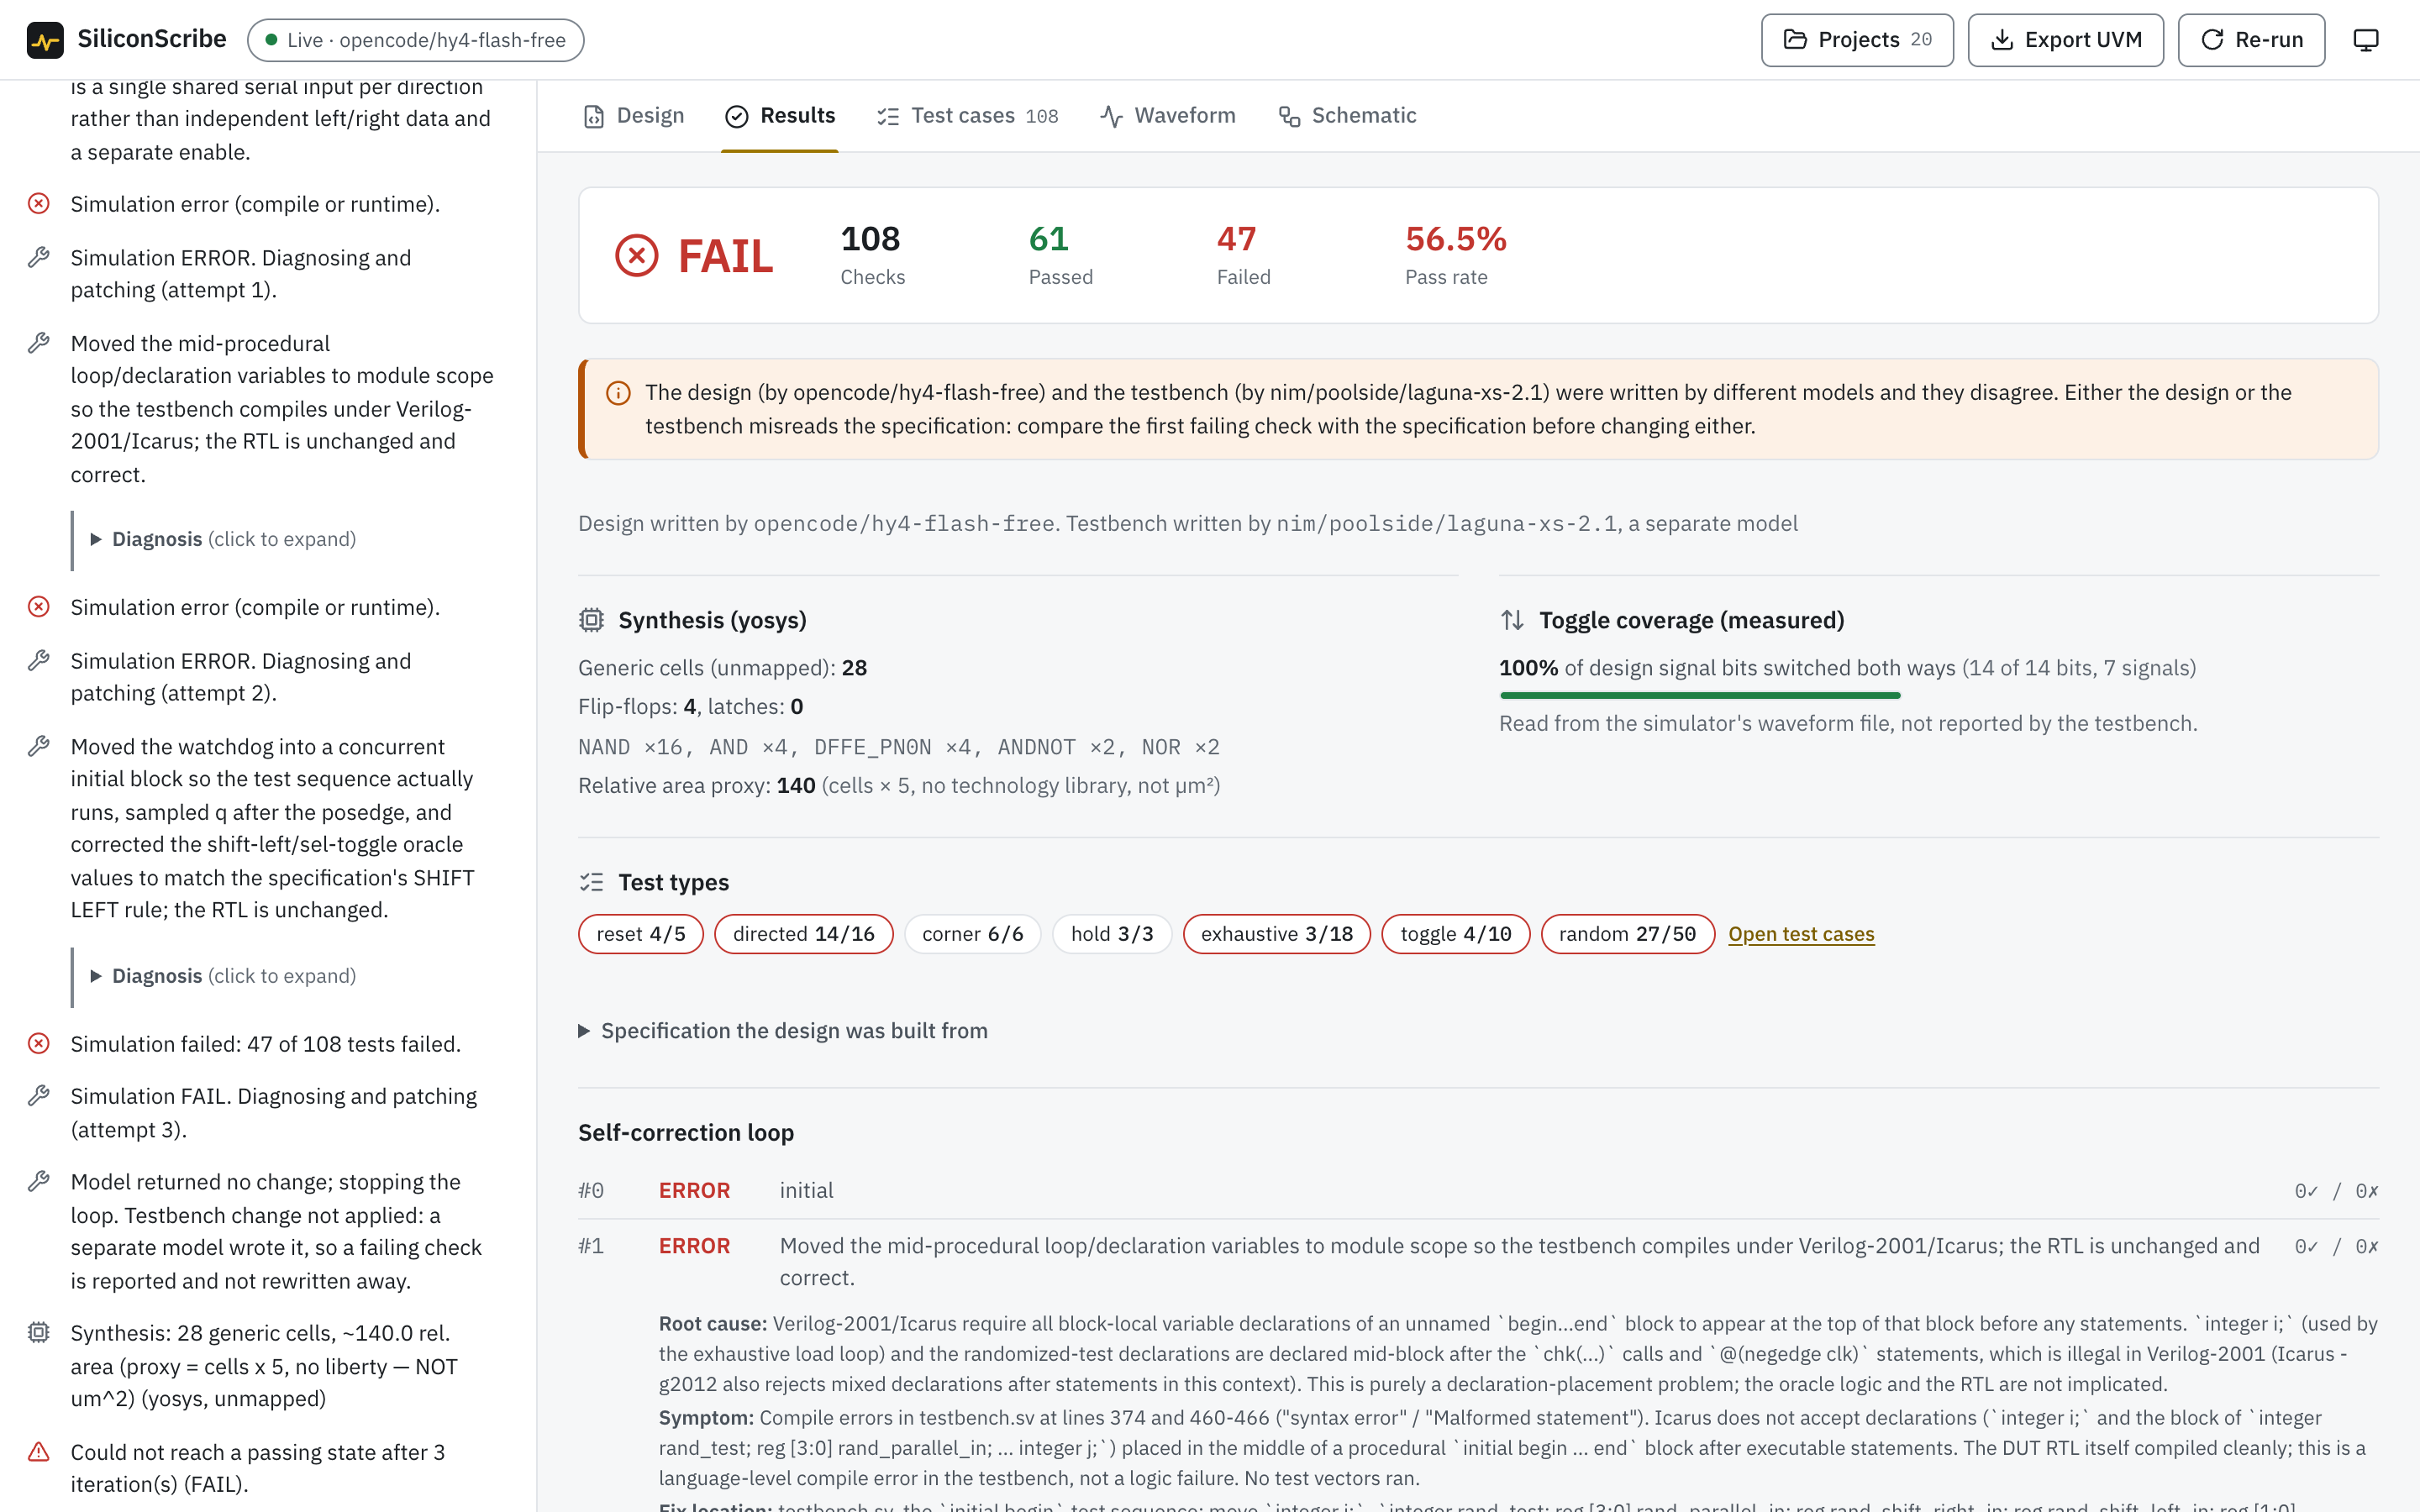
\includegraphics[width=0.85\textwidth]{s17_independent_testbench_fail.png}
\caption[A separate testbench model disagrees with the design]{Live run with the design by \texttt{opencode/hy4-flash-free} and the testbench by a separate model, \texttt{nim/poolside/laguna-xs-2.1}: FAIL 61/108 and the warning that the two models disagree. The run timeline (left) states that the testbench change was not applied. The testbench was later found to be the side at fault.}
\label{fig:indepfail}
\end{figure}

\subsection{Specification review and second opinion}
The s2 prompt (8-bit loadable up/down counter) was run with
\code{opencode/hy4-flash-free} and ``Review the specification before generating''
ticked (Figure~\ref{fig:specreview}). The confirmed specification was used exactly.
The run reached PASS (8672 of 8672 checks) after one repair, but that repair rewrote
the testbench, so a fresh testbench was generated from the same specification as a
second opinion. It also passed (8517 of 8517) and agreed with the final design, while
the original testbench still failed on the final design (1038 failed checks), which
was shown as a warning on the PASS (Figure~\ref{fig:second}). A hand-written reference
model then gave 0 mismatches in 40,027 cycles: the design was correct and the original
testbench was wrong.

The same behaviour was seen on a live FIFO run, also by
\code{opencode/hy4-flash-free}. The run passed 4134 of
4134 checks after one repair that changed the testbench; the second-opinion testbench
passed all 3798 of its checks, while the original testbench still reported 482 failed
checks on the final design. Since the fourth review round such a run is shown as
``PASS, disputed'' in warning colour rather than as a plain PASS (Figure~\ref{fig:second},
the recorded run replayed in the current interface). The same
results panel also shows the strength (11 of 12 injected bugs caught), the timing and
area estimate and the measured toggle coverage (100\%, 31 of 31 bits).

\begin{figure}[htbp]
\centering
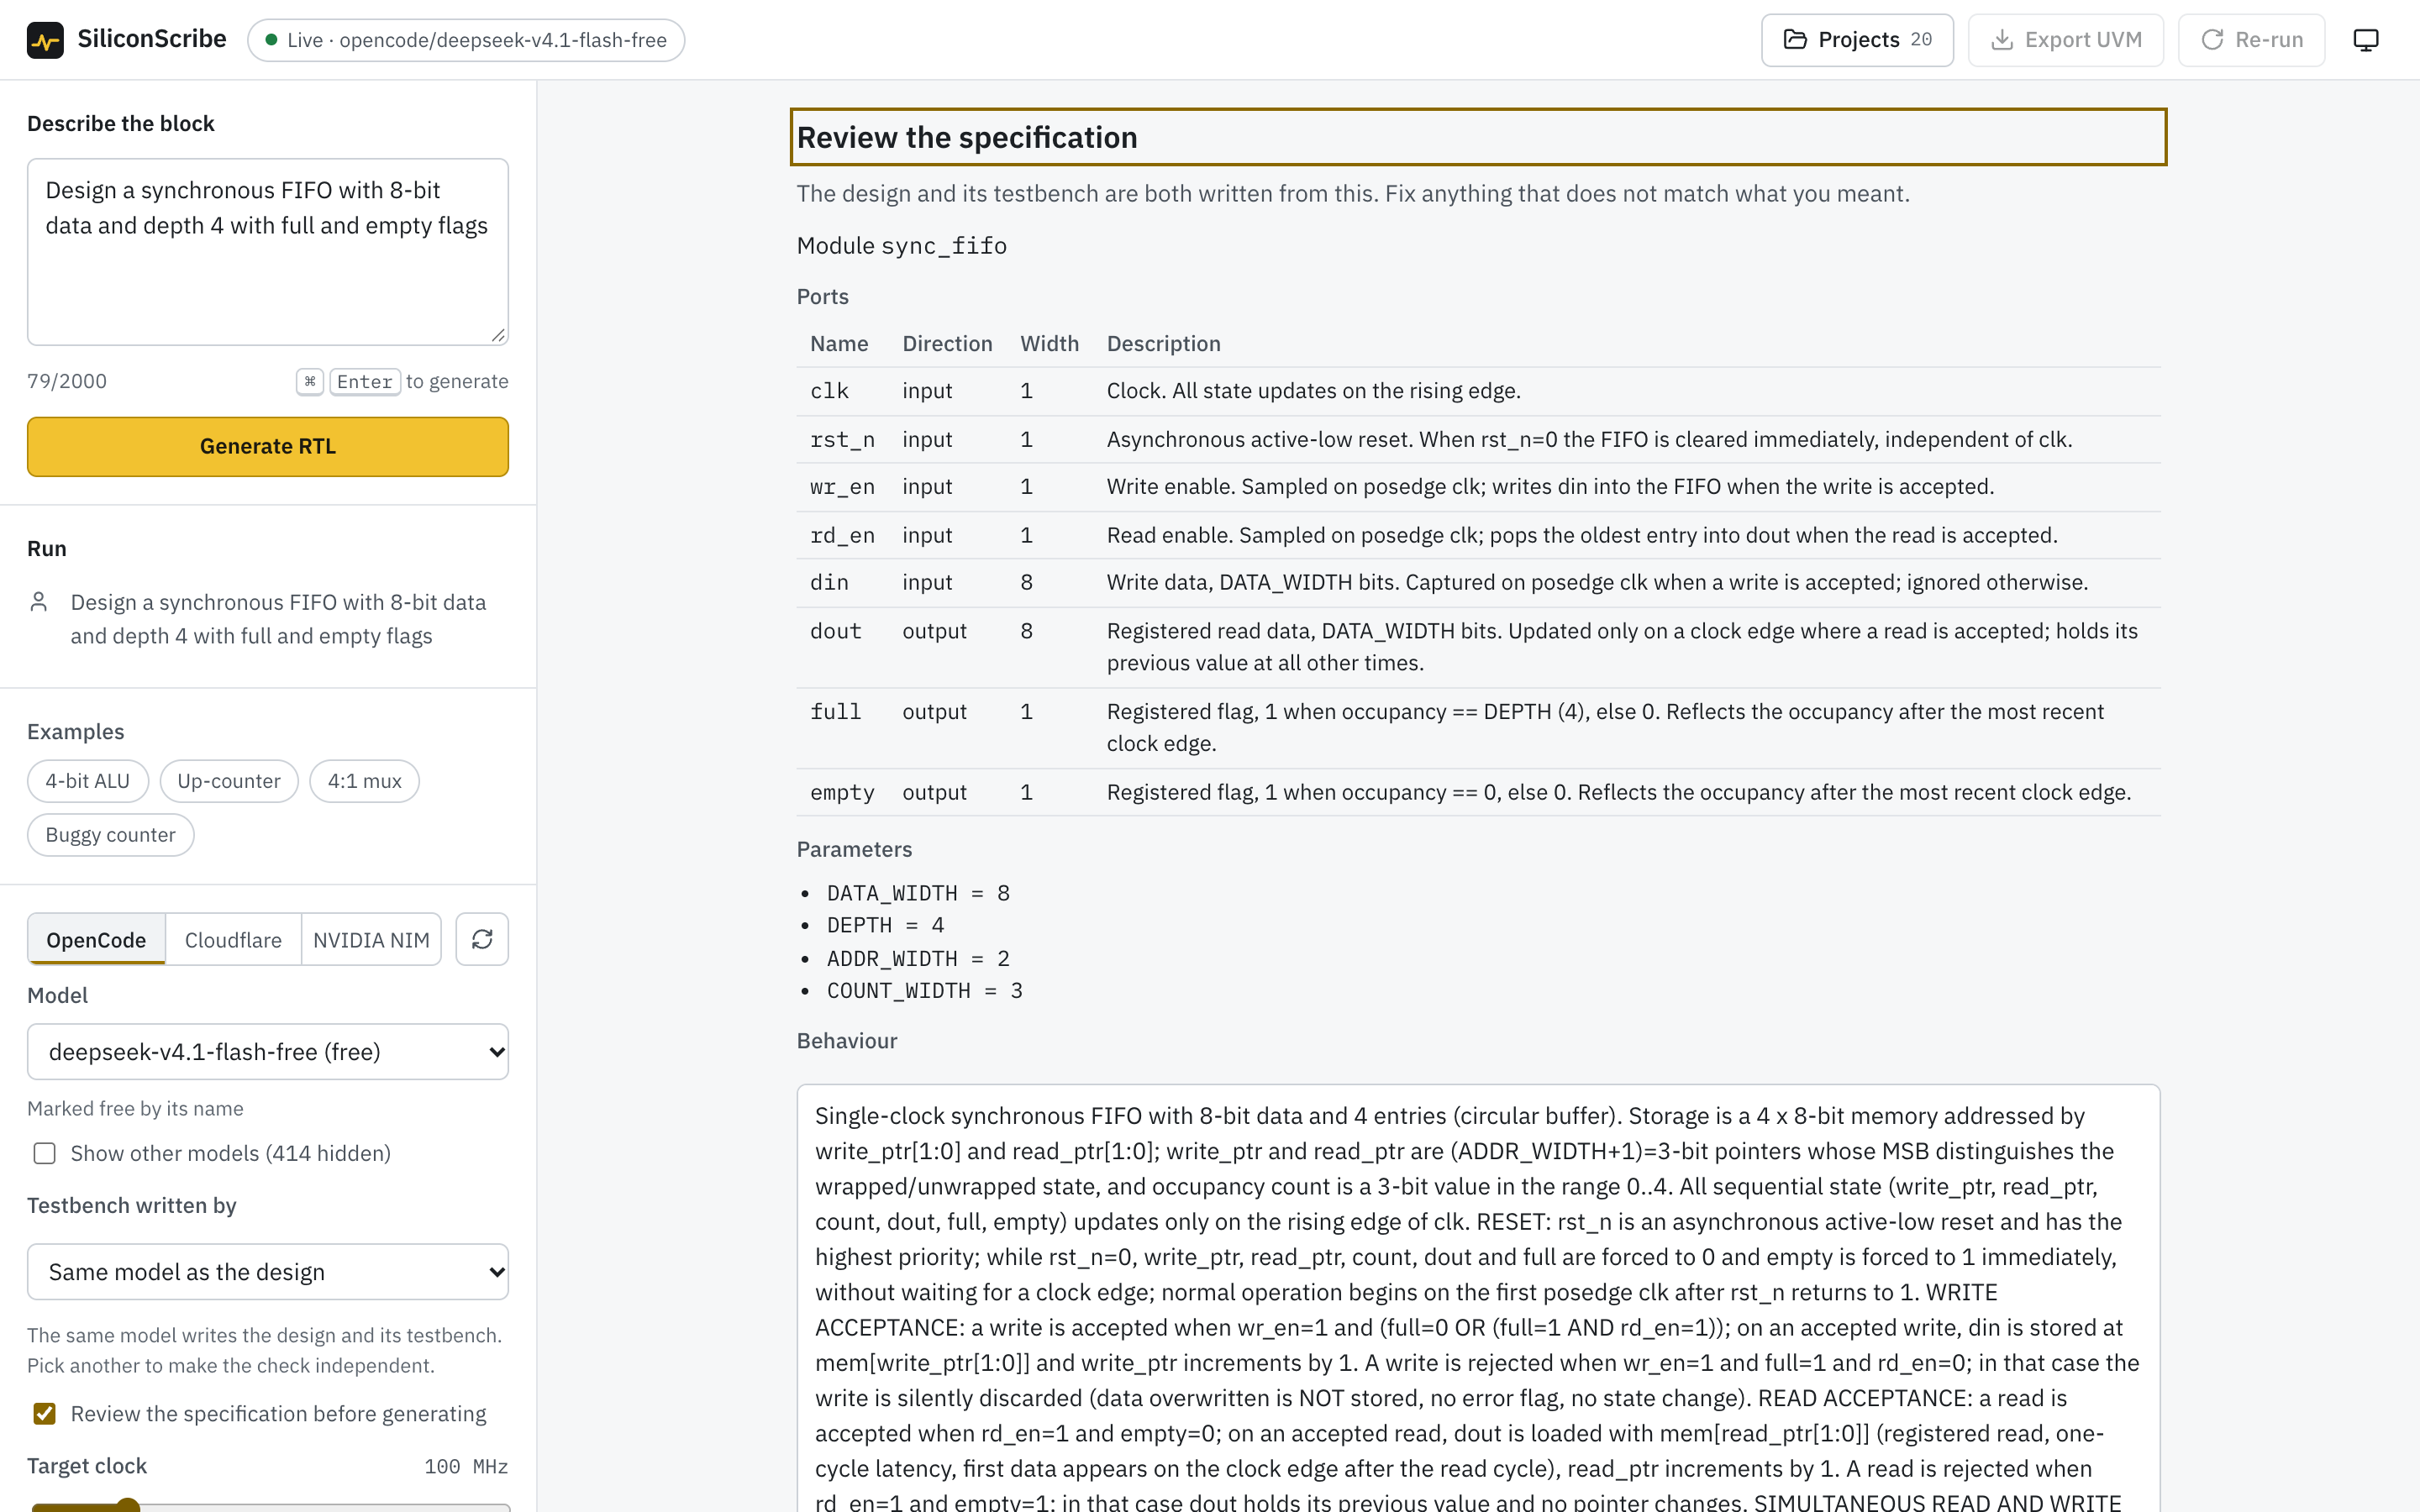
\includegraphics[width=0.7\textwidth]{s04_spec_review.png}
\caption[Specification review before generation]{Reviewing the parsed specification before generation. The specification shown was written by the live model for the FIFO prompt: ports table and editable behaviour and constraints.}
\label{fig:specreview}
\end{figure}

\begin{figure}[htbp]
\centering
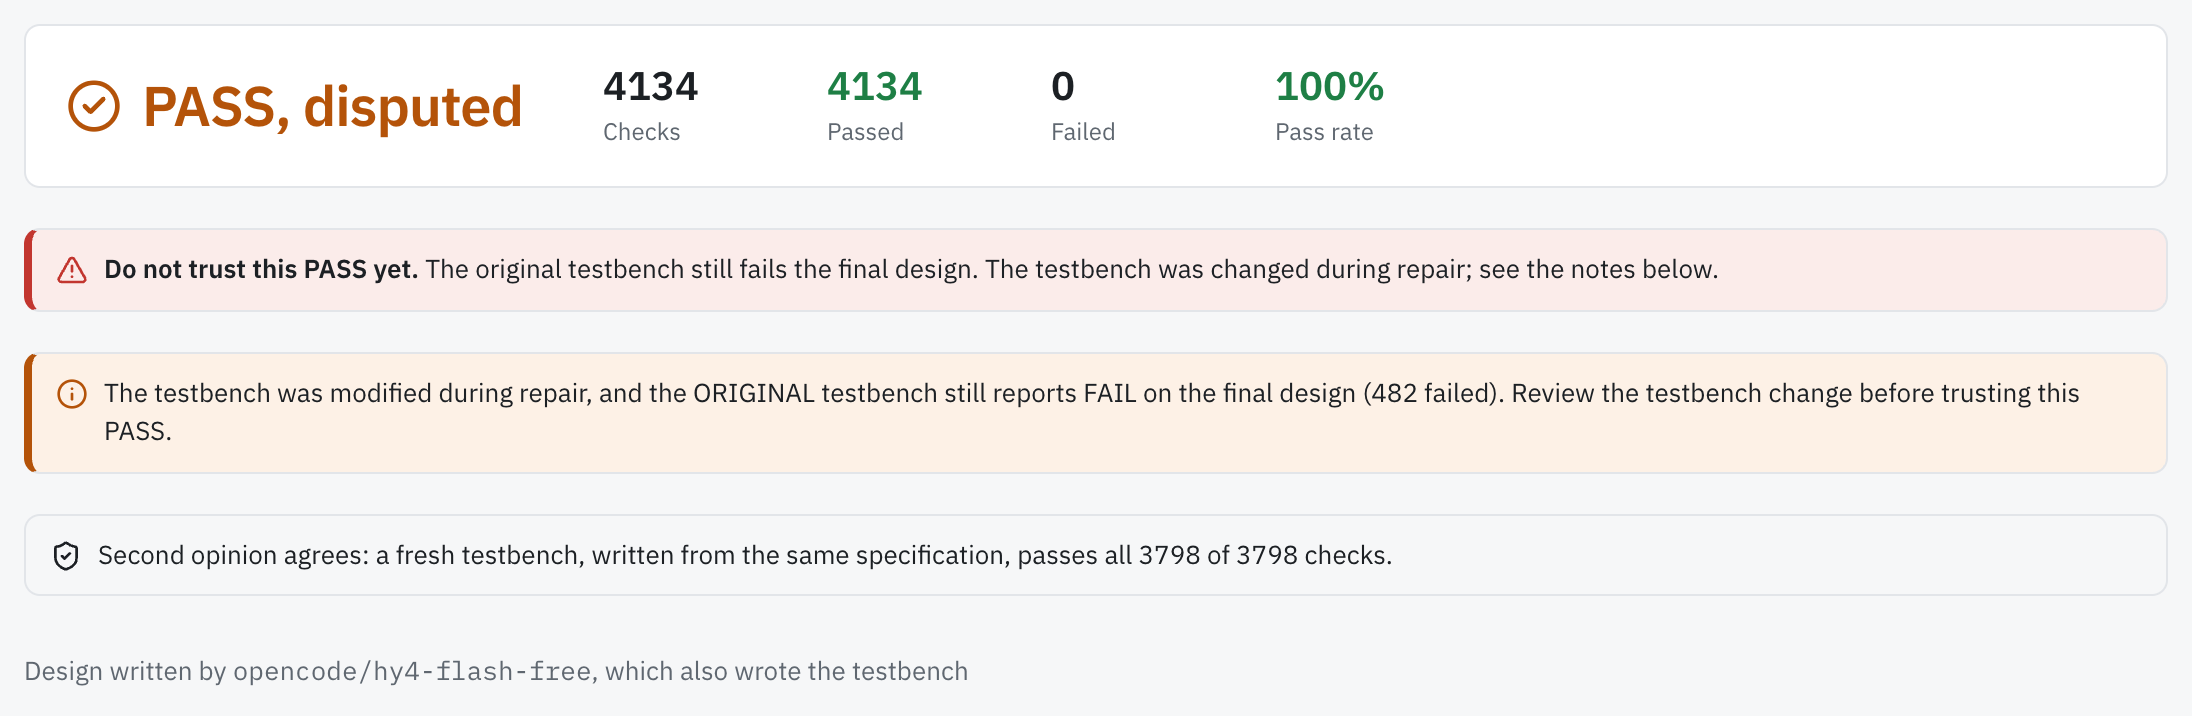
\includegraphics[width=0.85\textwidth]{s08_second_opinion.png}
\caption[Disputed PASS on a live run]{Top of the results panel of a live FIFO run by \texttt{opencode/hy4-flash-free} (close-up, the recorded run replayed in the current interface): the simulator's PASS 4134/4134 after one repair is shown as ``PASS, disputed'' because the original testbench still fails the final design (482 failed); the fresh second-opinion testbench agrees (3798/3798).}
\label{fig:second}
\end{figure}

\section{Early Live Run: Priority-Encoder Prompt}
The first version of the system was validated on the following prompt, which is
also prompt c1 of the evaluation above:

\begin{quote}
\itshape ``Design an 8-to-3 priority encoder with an active-high valid output. Input
in[7:0]; outputs code[2:0] and valid. The highest set bit wins: bit 7 $\rightarrow$
code 7, bit 6 $\rightarrow$ code 6, \ldots, bit 0 $\rightarrow$ code 0. When in is
zero, code=0 and valid=0. Purely combinational.''
\end{quote}

Live provider: OpenRouter, model \code{nvidia/nemotron-3-ultra-550b-a55b:free},
timeout 180~s, reasoning disabled. The browser run produced \textbf{105/105 checks,
0 failed, PASS, 0 repair iterations}, with no degraded-mode banner. A second headless
run of the same prompt produced \textbf{116/116 checks} (the generated random loop
bound differs slightly between runs), also PASS on the first attempt. The model
generated a \code{casez} priority chain (archived as
\code{docs/evidence/livepriority08_design.sv}); the testbench
combined directed corner cases with randomized vectors (the archived testbench in
Appendix~\ref{app:tb} uses 16 directed cases and 100 random vectors), so it is a
strong but not exhaustive check of the 256 possible inputs. This run predates the
strength, coverage and timing stages.

\section{Live Fault Diagnosis and Repair}
Passing a correct design is necessary but not sufficient. The diagnostic path was
validated by injecting a known semantic bug into a counter and running the
\emph{live} fixer with the \emph{independent} testbench. This is not the scripted
offline fix: the LLM received the RTL, the testbench, the specification, and the
simulator log, and returned a structured diagnosis.

\begin{table}[H]
\centering
\caption{Live fault-injection result (real LLM diagnosis, real simulator).}
\label{tab:seeded}
\small
\begin{tabularx}{\textwidth}{@{}l c c c X@{}}
\toprule
 & \textbf{Passed} & \textbf{Failed} & \textbf{Status} & \textbf{Action} \\
\midrule
Before & 1 & 19 & \textcolor{failred}{\textbf{FAIL}} & initial buggy RTL (\code{count + 2'd2}) \\
After  & 20 & 0 & \textcolor{passgreen}{\textbf{PASS}} & LLM diagnosis + RTL patch (\code{count + 1'b1}) \\
\bottomrule
\end{tabularx}
\end{table}

The fixer's diagnosis, quoted from the live response, was:

\begin{quote}
\footnotesize
\textbf{Symptom:} The testbench expects the counter to increment by 1 each cycle
(expected sequence: 1,2,3...), but the actual output increments by 2 (got sequence:
2,4,6...). The first failure is at expected=1, got=2.\\
\textbf{Root cause:} In the RTL, the counter increments by \code{2'd2} (i.e., 2)
when enable is asserted, but the specification requires a standard up-counter that
increments by 1.\\
\textbf{Fix location:} \code{counter.v} line 10 (the line
\code{count <= count + 2'd2;}).\\
\textbf{Confidence:} high.
\end{quote}

The model identified the \emph{actual} wrong line from the first failing vector, not
a generic ``counter is broken'' fallback. The testbench was not weakened; it was the
same independent testbench before and after the fix.

\section{Self-Correction in the Application}
The built-in ``buggy 4-bit counter'' demonstration shows the loop as the user sees
it. It uses the offline provider, so the repair is the labelled scripted path rather
than an LLM diagnosis (the live LLM diagnosis is Table~\ref{tab:seeded}). On the
current 57-check counter testbench the buggy RTL fails 48 of the 57 checks, and each
failed check is marked on the waveform (Figure~\ref{fig:failwave}) and listed in the
Test cases tab. The iteration timeline records every attempt, and for a scripted fix
the interface states that no root-cause diagnosis was produced instead of inventing
one.

\begin{figure}[htbp]
\centering
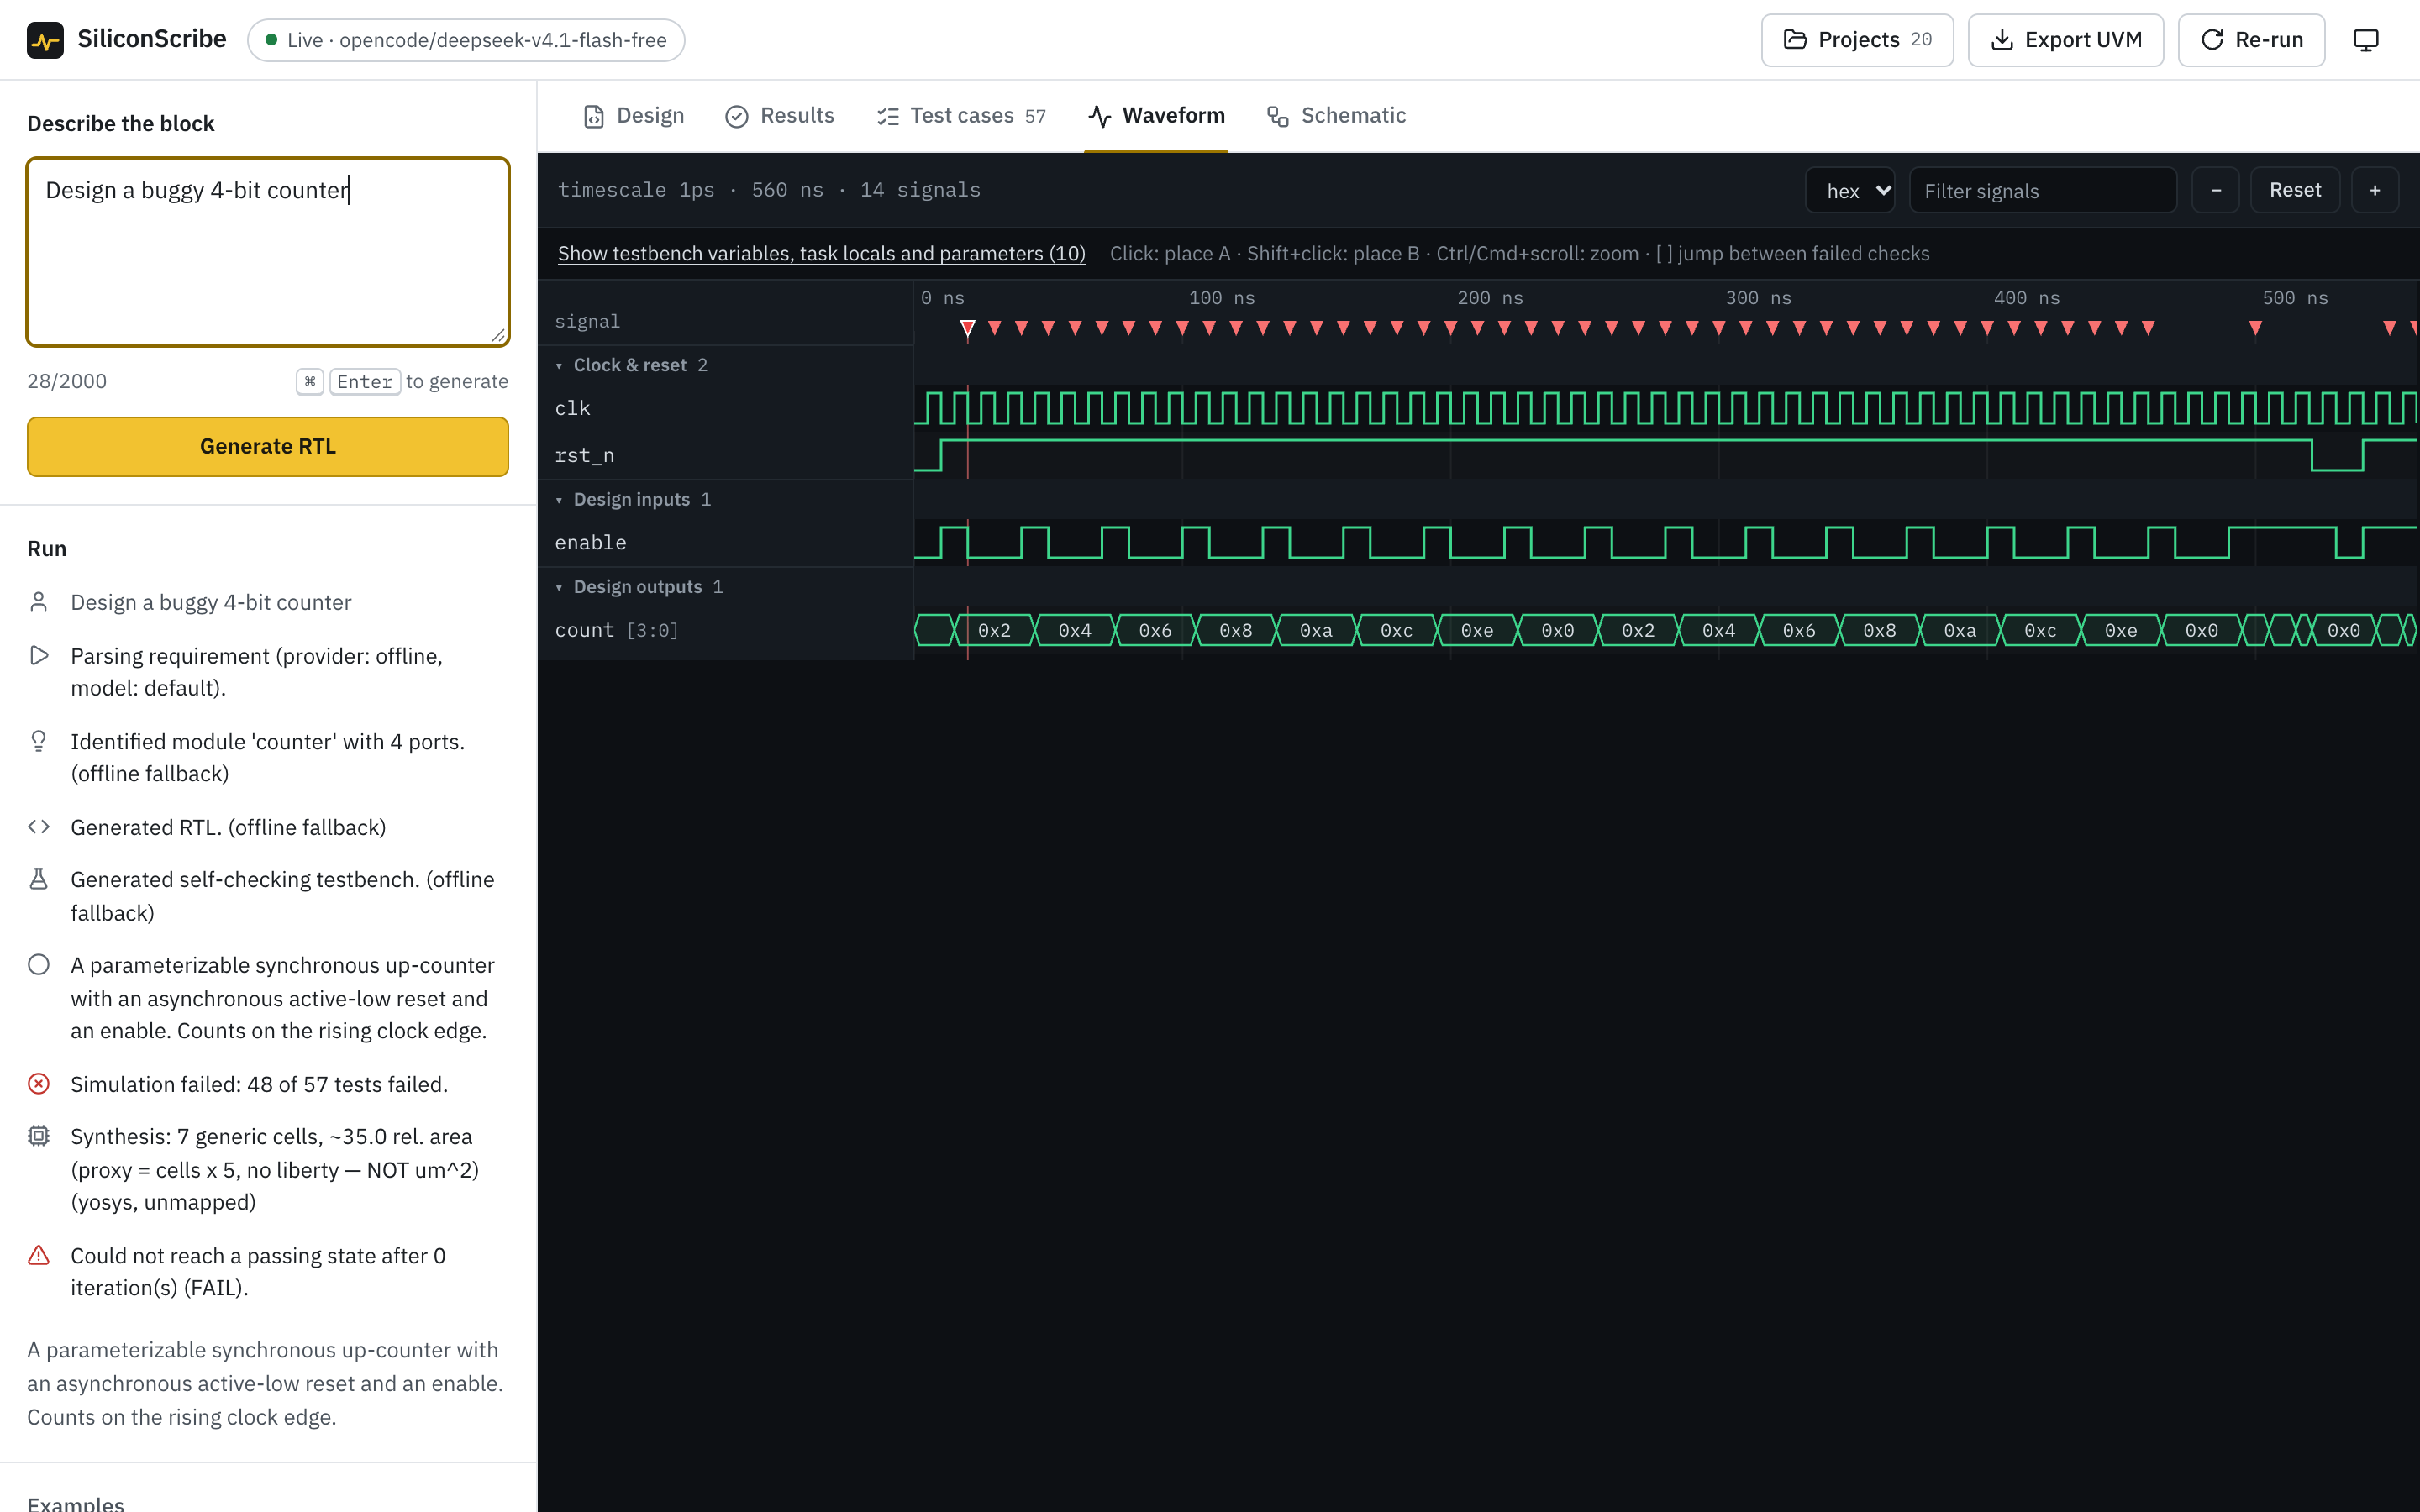
\includegraphics[width=0.7\textwidth]{s13_failure_waveform.png}
\caption[Waveform of the scripted buggy-counter demonstration]{Waveform of the scripted buggy-counter demonstration (offline): each red marker is a failed check (48 of 57).}
\label{fig:failwave}
\end{figure}

\section{Compiler-Repair Coverage}
Two mechanical repairs are covered by unit tests that run real Icarus:

\begin{itemize}
\item a testbench-level \code{wire} assigned in an \code{initial} block is changed
to \code{reg}, with a diagnosis naming \code{testbench.sv} and the signal;
\item a \code{disable <function>} early return is changed to
\code{return <function>}, preserving first-match semantics.
\end{itemize}

Both tests assert that the fixer LLM is \emph{not} called for a mechanical repair,
and that the subsequent simulation reaches PASS.

\section{Mutation Sweep: Can the Testbenches Fail?}
A testbench that passes everything is not evidence, so its strength was measured. One semantic bug at a time was injected into the golden RTL of each curated design and the curated testbench was required to turn PASS into FAIL. The first sweep killed 11 of 14 mutants; the three survivors were genuine testbench gaps: the counter testbench never turned \code{enable} off (so a counter that ignores \code{enable} passed), and the ALU testbench neither checked the \code{overflow} flag nor drove the undefined opcodes 5 to 7. The testbenches were then hardened (Table~\ref{tab:mutants}) and the sweep re-run.

\begin{table}[H]
\centering
\caption{Mutation sweep over the curated designs: first sweep versus after hardening the testbenches.}
\label{tab:mutants}
\small
\begin{tabular}{@{}l l c c@{}}
\toprule
\textbf{Design} & \textbf{Injected bug} & \textbf{First sweep} & \textbf{After hardening} \\
\midrule
counter & increment by 2 & \textcolor{passgreen}{killed} & \textcolor{passgreen}{killed} \\
counter & decrement & \textcolor{passgreen}{killed} & \textcolor{passgreen}{killed} \\
counter & reset polarity inverted & \textcolor{passgreen}{killed} & \textcolor{passgreen}{killed} \\
counter & reset ignored & \textcolor{passgreen}{killed} & \textcolor{passgreen}{killed} \\
counter & wrong reset value & \textcolor{passgreen}{killed} & \textcolor{passgreen}{killed} \\
counter & enable ignored & \textcolor{failred}{\textbf{survived}} & \textcolor{passgreen}{killed} \\
ALU & AND replaced by OR & \textcolor{passgreen}{killed} & \textcolor{passgreen}{killed} \\
ALU & ADD replaced by SUB & \textcolor{passgreen}{killed} & \textcolor{passgreen}{killed} \\
ALU & SUB replaced by ADD & \textcolor{passgreen}{killed} & \textcolor{passgreen}{killed} \\
ALU & XOR replaced by OR & \textcolor{passgreen}{killed} & \textcolor{passgreen}{killed} \\
ALU & overflow stuck at 0 & \textcolor{failred}{\textbf{survived}} & \textcolor{passgreen}{killed} \\
ALU & undefined opcode not zero & \textcolor{failred}{\textbf{survived}} & \textcolor{passgreen}{killed} \\
full adder & sum drops carry-in & \textcolor{passgreen}{killed} & \textcolor{passgreen}{killed} \\
mux4to1 & d0 and d1 swapped & \textcolor{passgreen}{killed} & \textcolor{passgreen}{killed} \\
\midrule
\multicolumn{2}{@{}l}{\textbf{Mutants killed}} & \textbf{11 / 14} & \textbf{14 / 14} \\
\bottomrule
\end{tabular}
\end{table}

The counter testbench gained an enable-hold phase, an asynchronous-reset phase and a resume phase. In the second review round it was rewritten again so that every comparison is logged individually, and it now runs 57 checks of four types (reset, directed, hold, corner). The ALU testbenches now drive all eight opcodes and check the carry or borrow output against an independent wide-addition reference. The sweep is reproducible with \code{python3 tools/mutation_sweep.py}, and the regression suite pins 16 mutants. In the second review round the sweep was extended to 27 mutants, including the survivors an independent reviewer found, and all 27 are killed.

The sweep uses hand-picked bugs on the built-in designs. Since then the same idea runs automatically inside the application on every PASS, with up to 12 generated one-token mutants (Section~\ref{sec:trustimpl}). On the built-in counter it catches 7 of 8; the survivor, \code{posedge} changed to \code{negedge}, is a genuine small blind spot of the counter testbench, whose sampling cannot tell the two clock edges apart (Figure~\ref{fig:degraded}).

\section{Supporting Outputs}
The application also produces a schematic in three views, a three-tier lint report,
Yosys generic-cell counts, the sky130 timing and area estimate, a bounded VCD
waveform, and a 16-file UVM 1.2 export. The UVM bundle is export-only: Icarus cannot
compile UVM, so it is never simulated. Figure~\ref{fig:cwave} shows the waveform viewer.
Figures~\ref{fig:schrtl} and~\ref{fig:schgate} show the RTL-cell and gate-level
schematic views; the block diagram view shows only the ports. Both netlist views are
drawn from the Yosys netlist of the run that is on screen. The gate-level view uses
Yosys' generic gates, not the sky130 cells that are timed.

\begin{figure}[htbp]
\centering
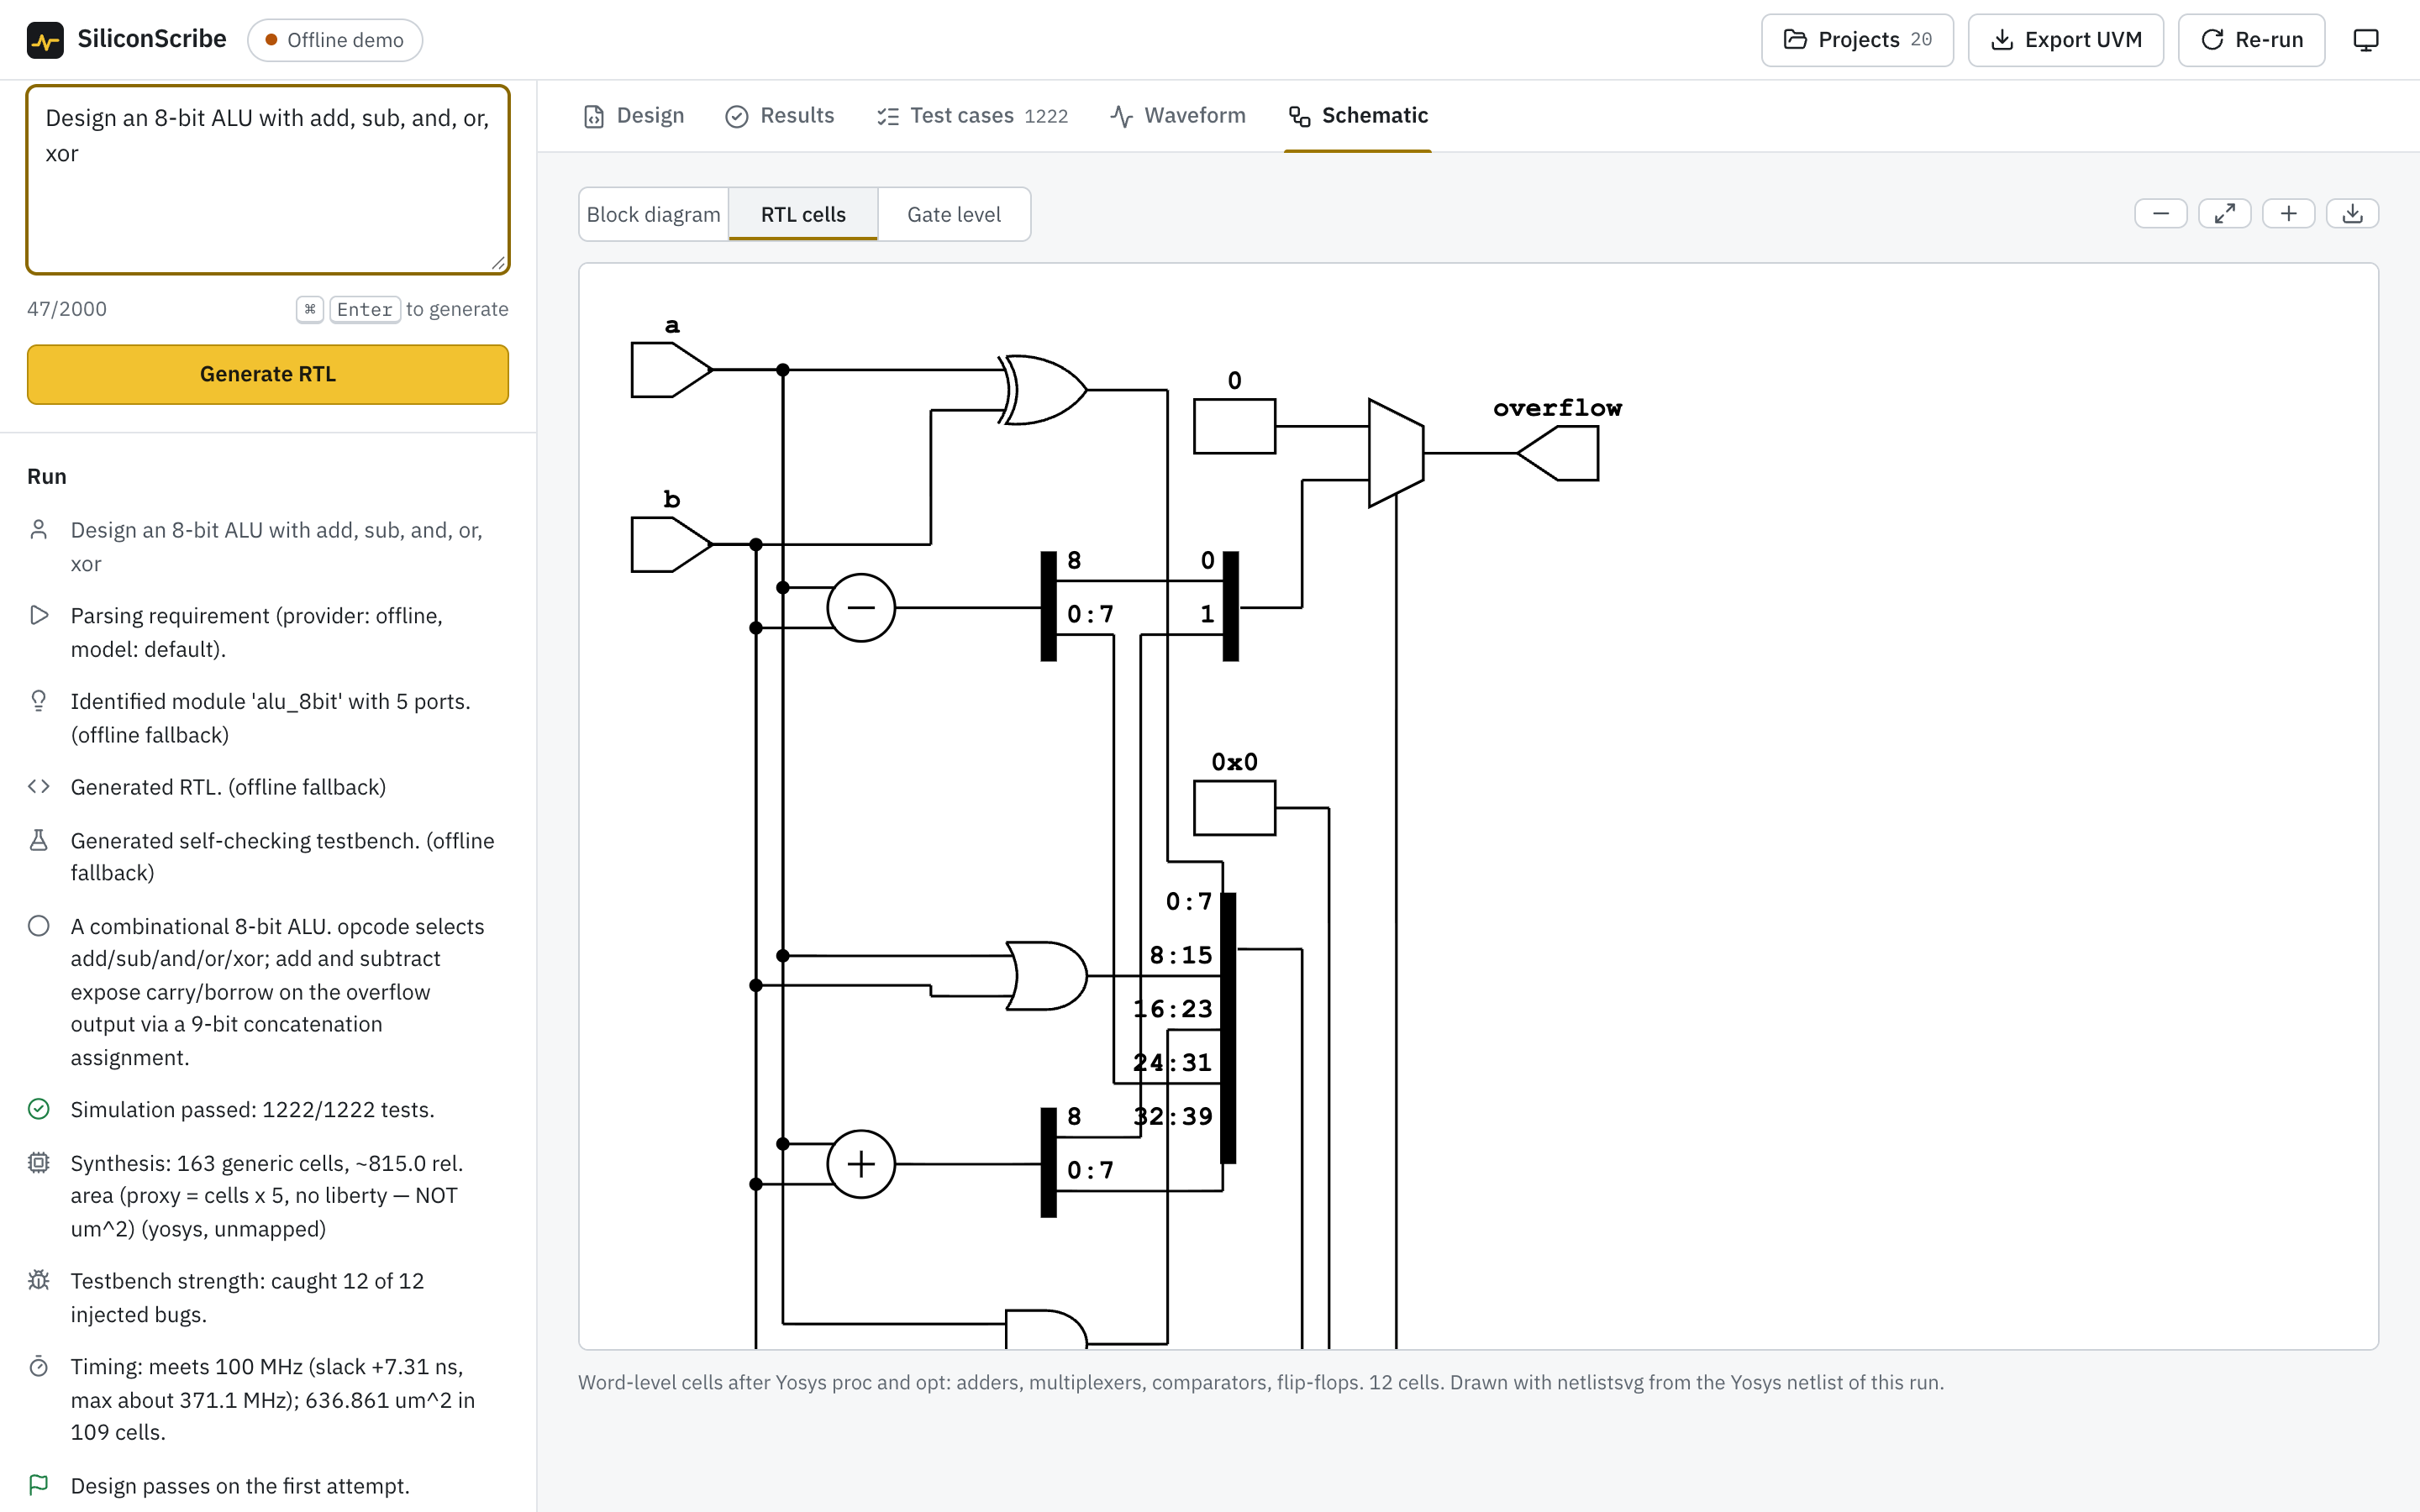
\includegraphics[width=0.7\textwidth]{s18_schematic_rtl_cells.png}
\caption[RTL cells view of the schematic tab]{Schematic tab, ``RTL cells'' view of the \emph{built-in} 8-bit ALU (offline demo design, labelled ``Offline demo'' in the header): subtractor, adder, XOR, AND and OR cells, a multiplexer and bus splits (12 cells), drawn with netlistsvg from the Yosys netlist of the run.}
\label{fig:schrtl}
\end{figure}

\begin{figure}[htbp]
\centering
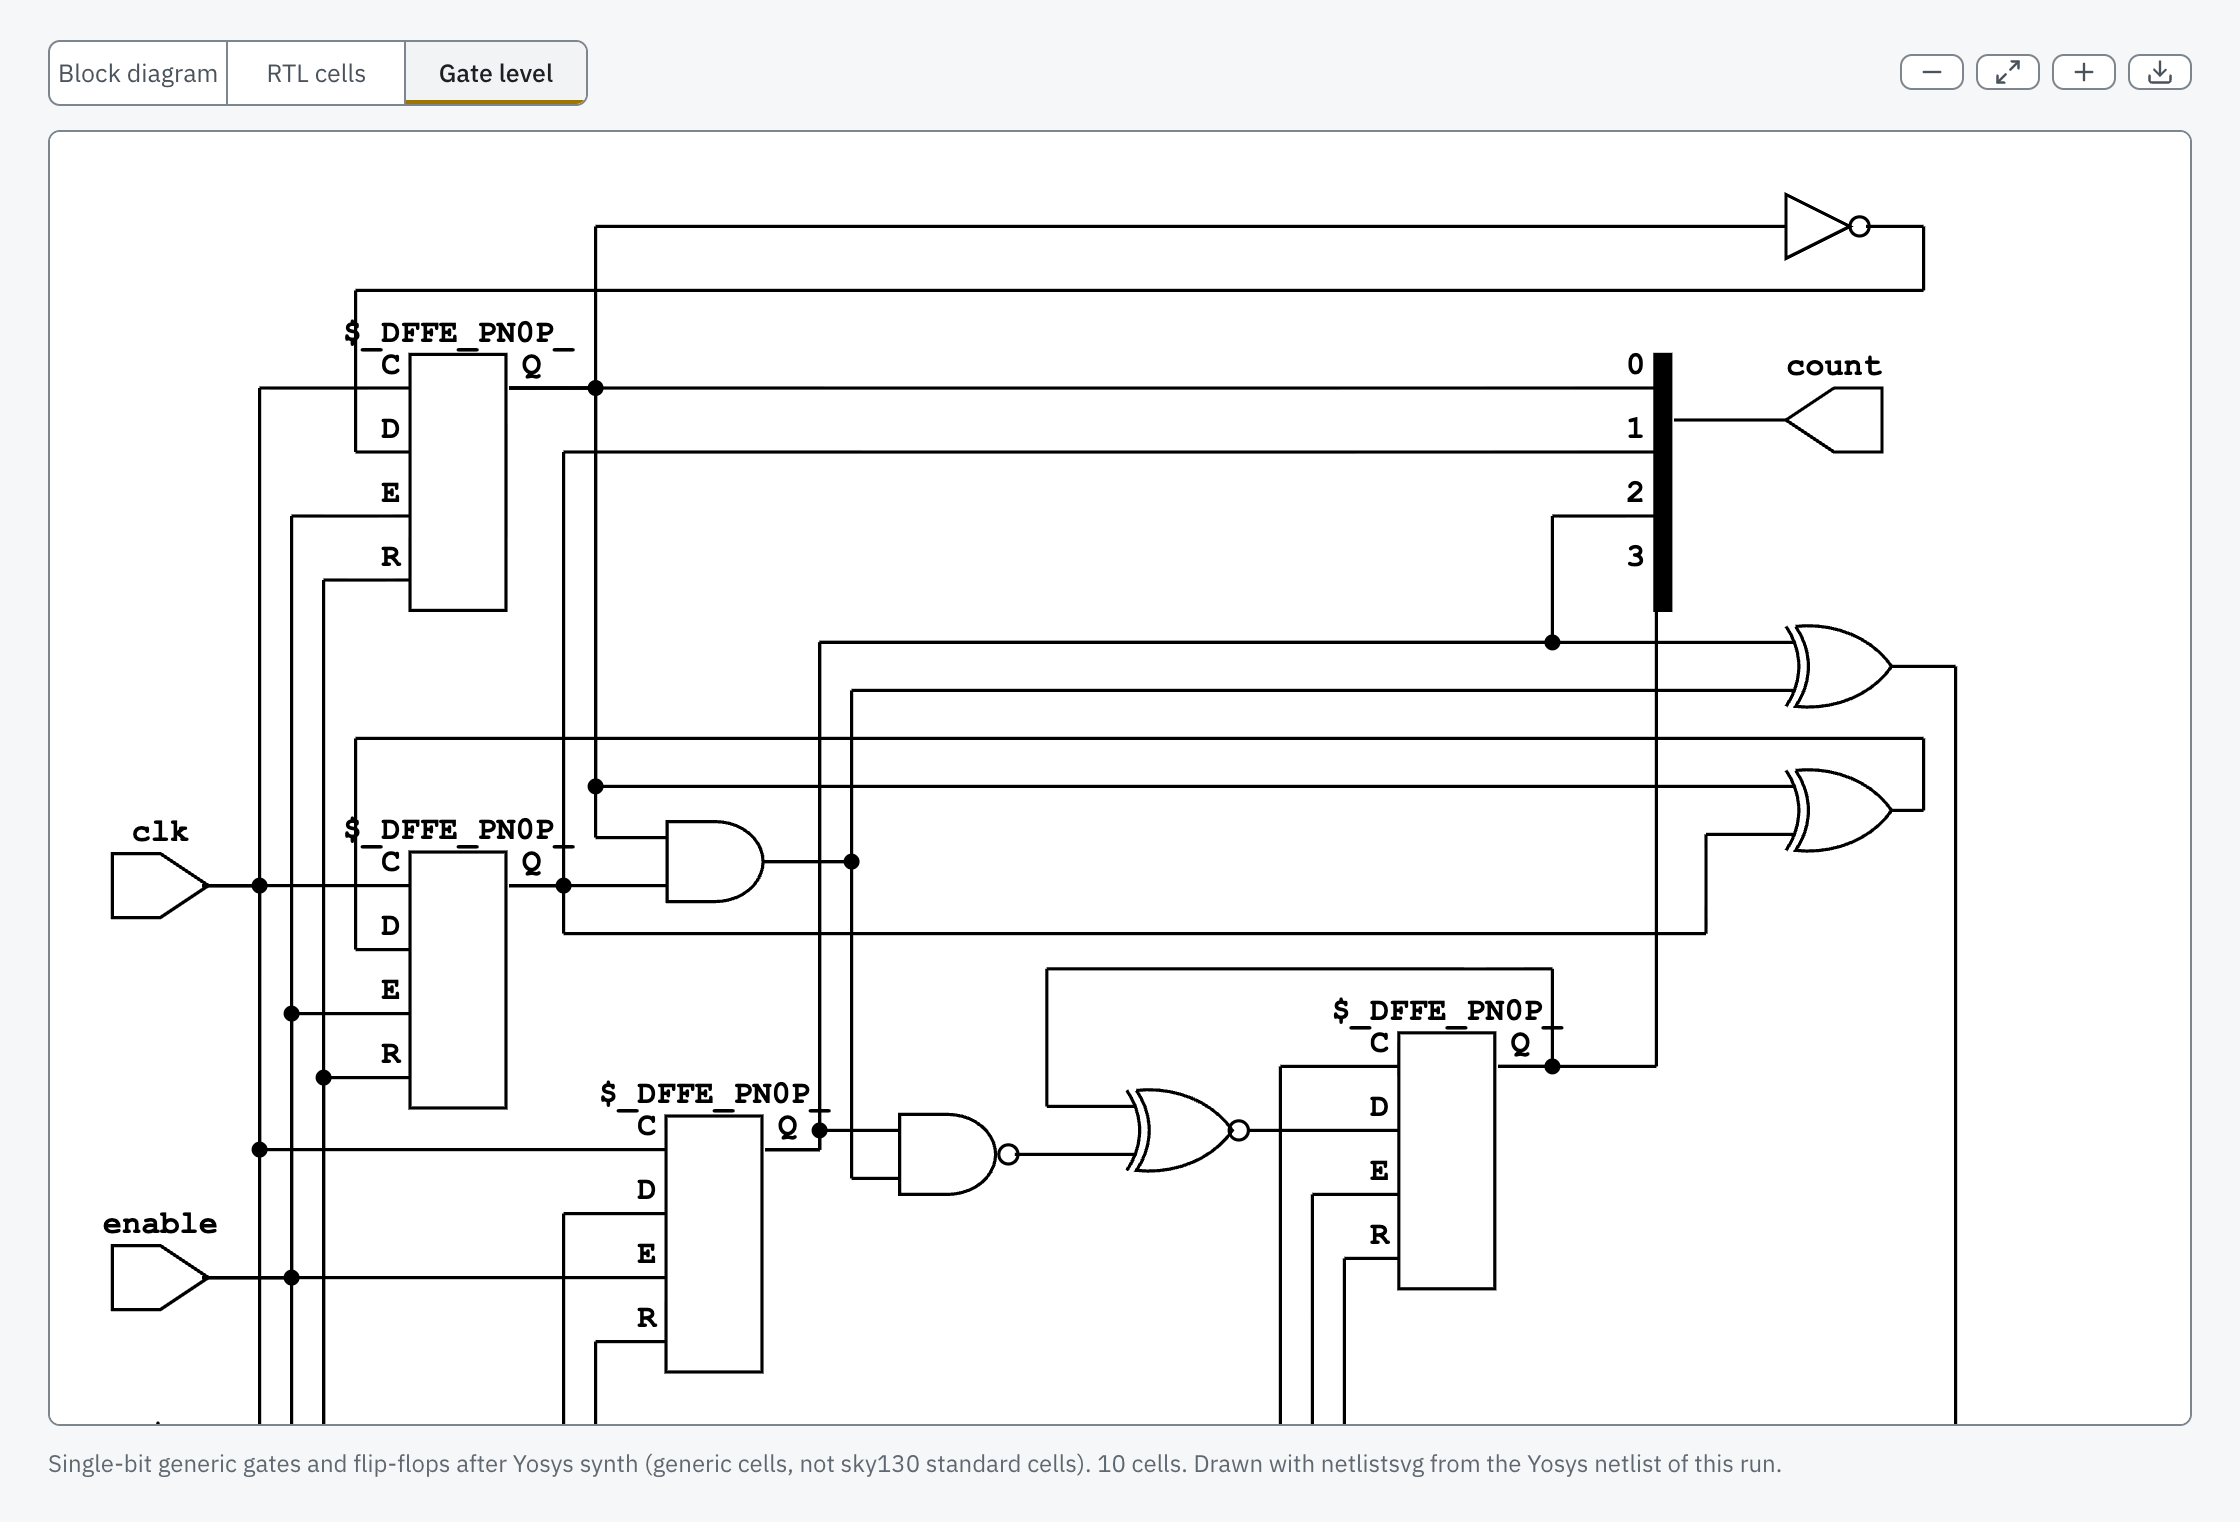
\includegraphics[width=0.7\textwidth]{s19_schematic_gate_level.png}
\caption[Gate level view of the schematic tab]{Schematic tab, ``Gate level'' view of the \emph{built-in} 4-bit counter (offline demo design): four enabled flip-flops with asynchronous reset and the XOR/NAND next-state logic. These are Yosys generic gates, not sky130 cells.}
\label{fig:schgate}
\end{figure}

\begin{figure}[htbp]
\centering
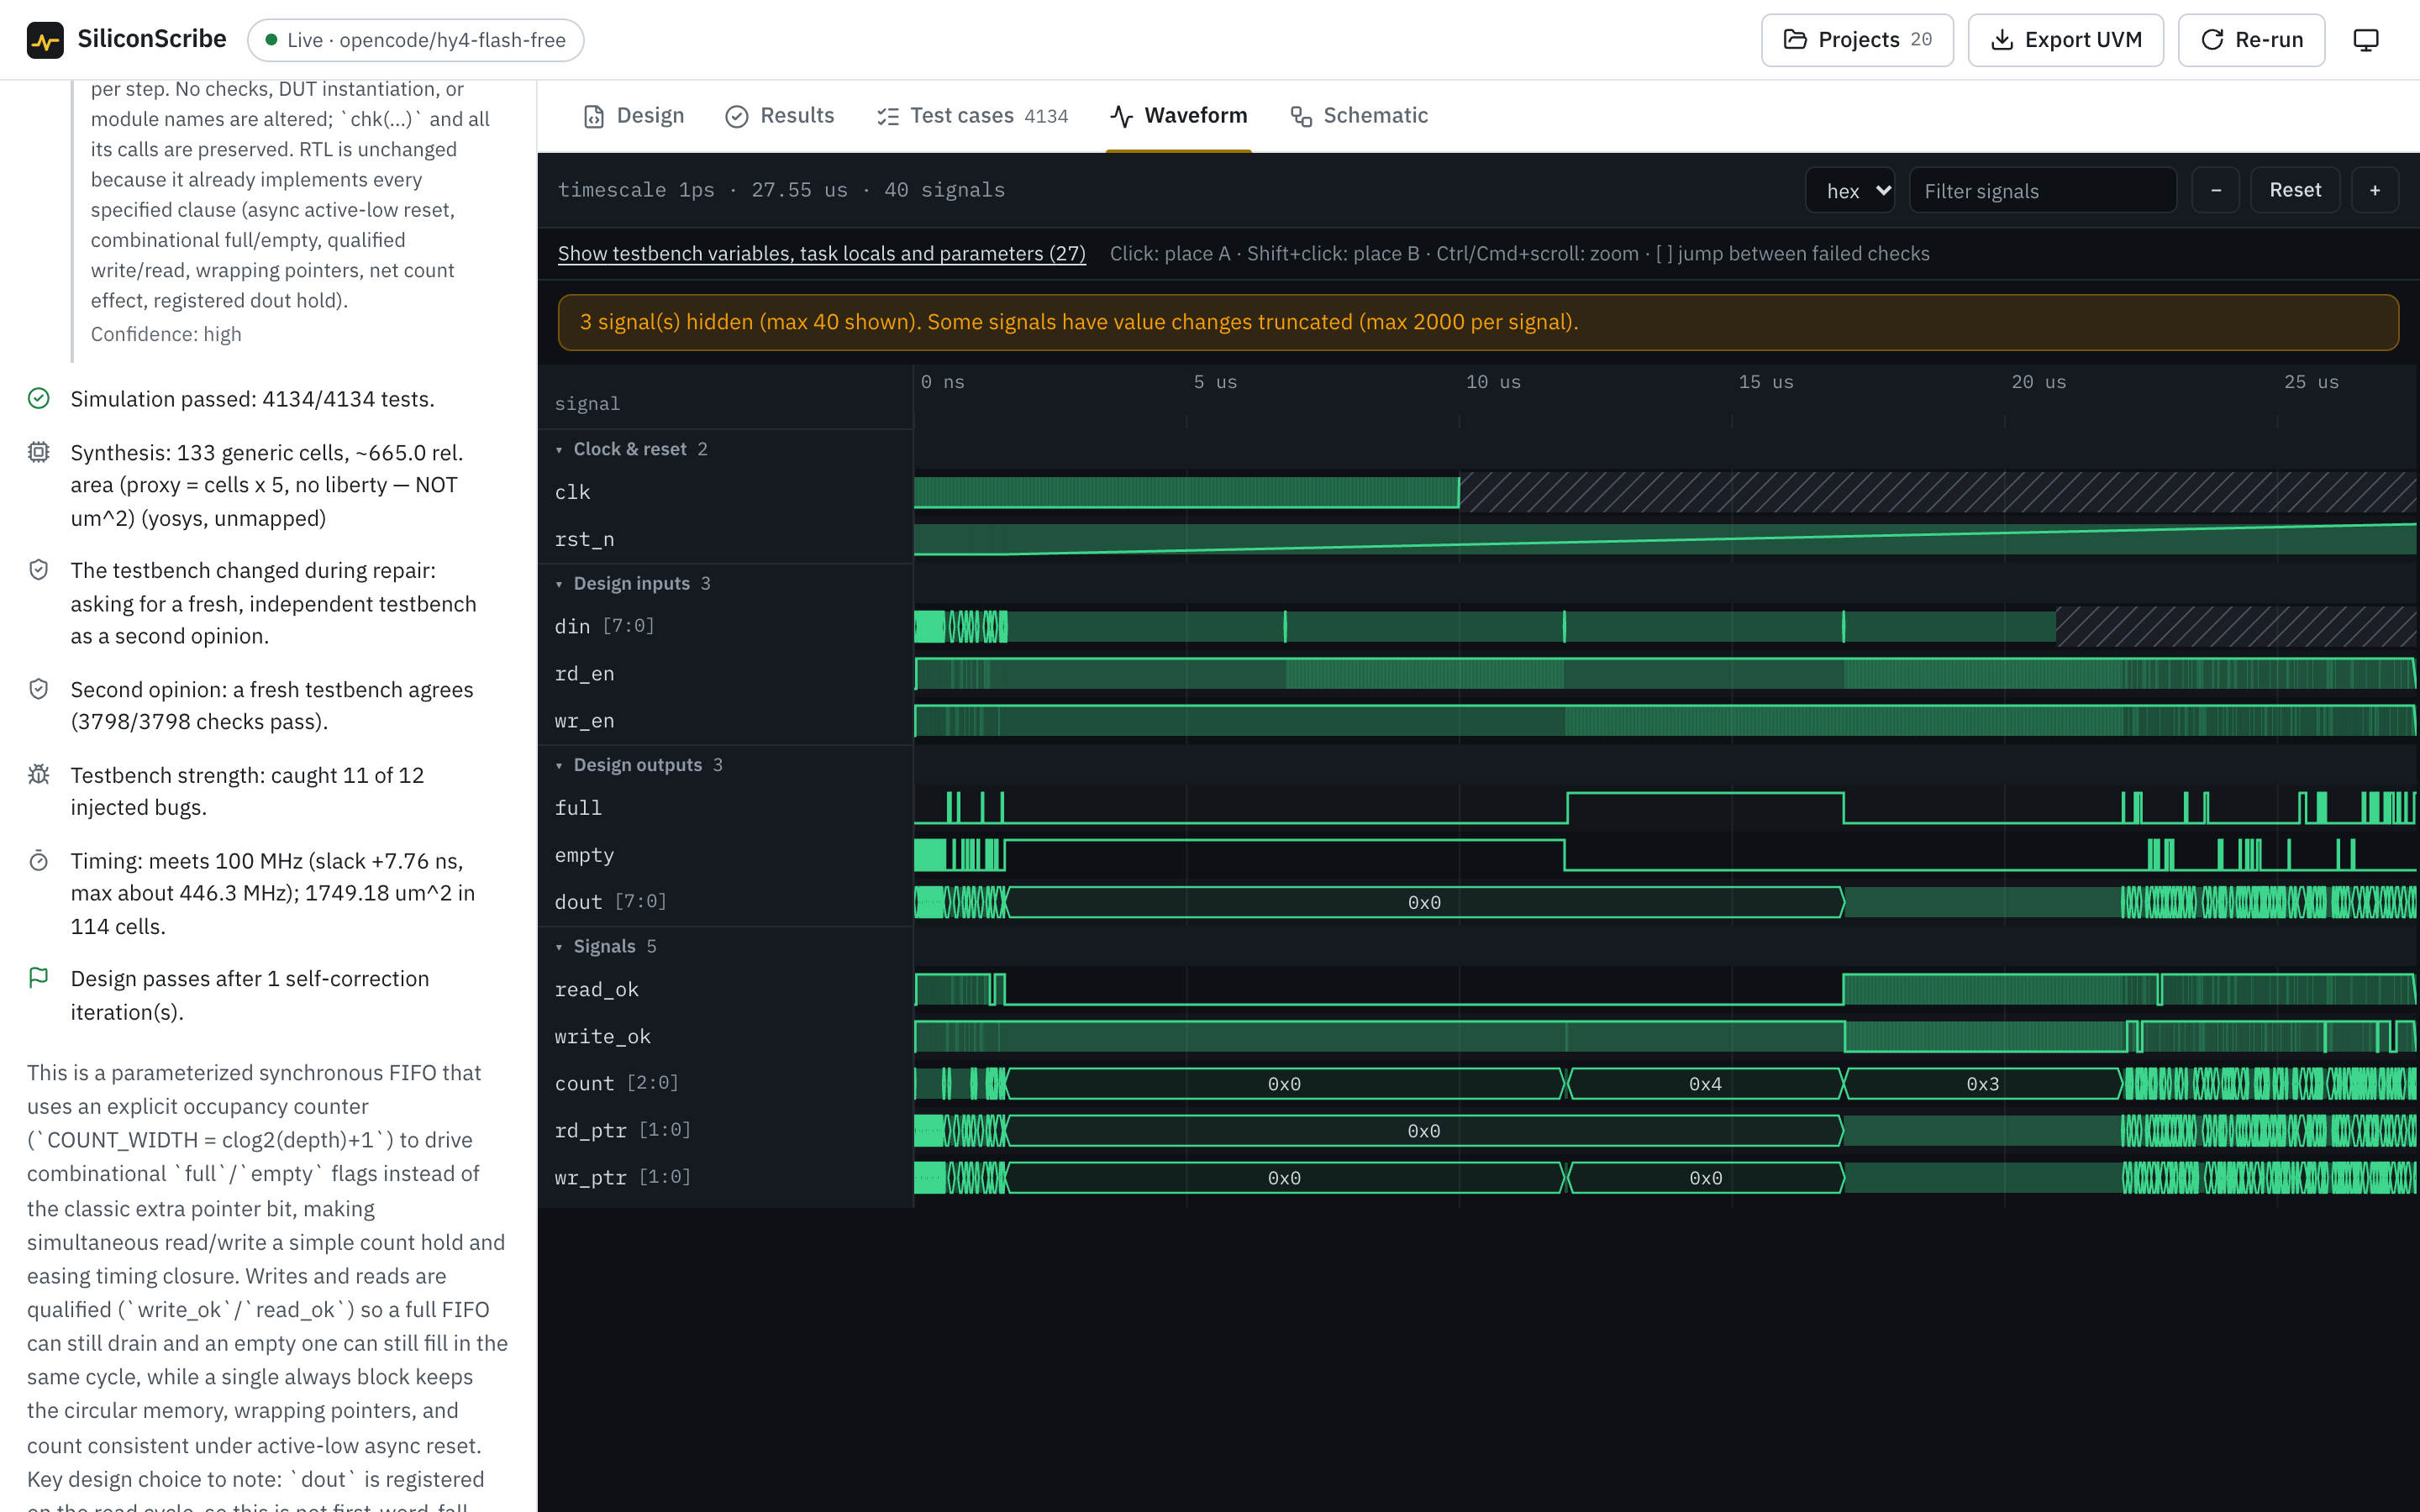
\includegraphics[width=0.7\textwidth]{s10_waveform.png}
\caption[Waveform tab of a live run]{Waveform tab of the live FIFO run, parsed from the simulator's VCD: signals grouped by role (clock and reset, design inputs, outputs, internal signals), hex radix, and a notice that some signals were hidden or truncated to keep the view bounded.}
\label{fig:cwave}
\end{figure}

\section{Project Persistence}
Finished runs are stored in SQLite and listed in the Projects menu with Load and Delete actions (Figure~\ref{fig:projects}). The first final review found that only the blocking route saved a project while the browser uses the streaming route, so nothing generated in the interface ever appeared in the list. The streaming route now persists the finished run, and a regression test pins it.

\begin{figure}[htbp]
\centering
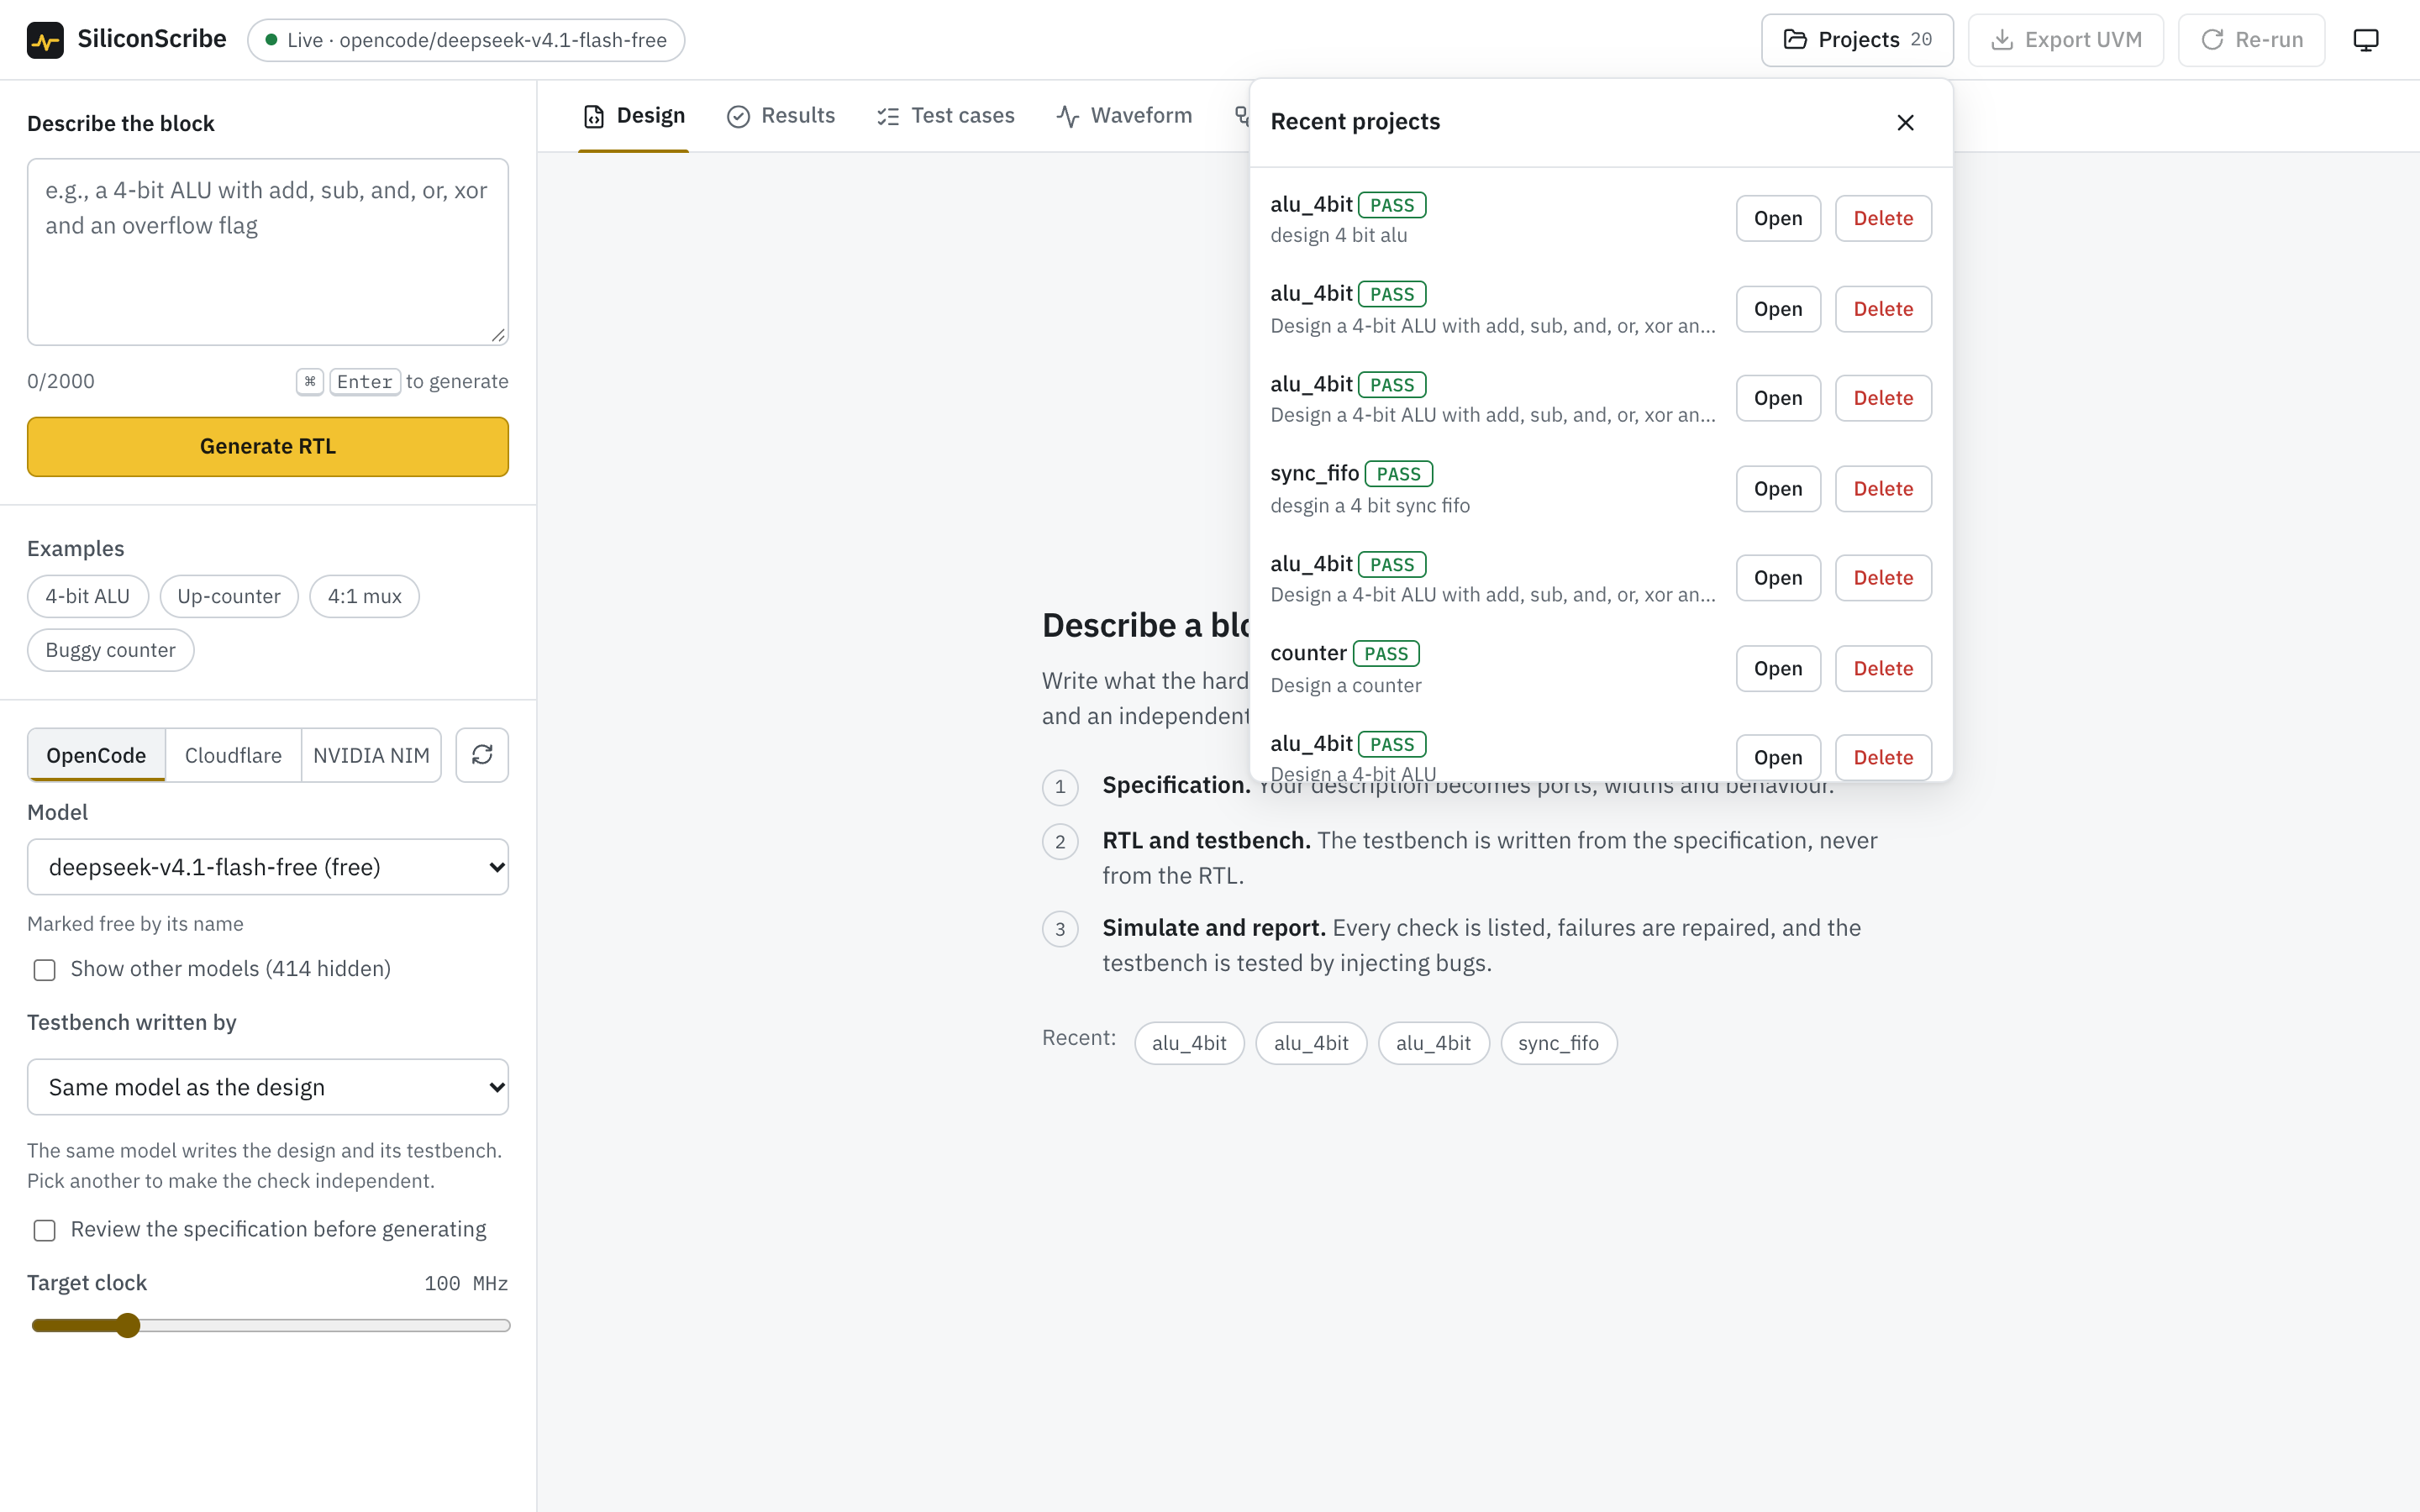
\includegraphics[width=0.5\textwidth]{s14_projects_menu.png}
\caption{The Projects menu listing saved runs.}
\label{fig:projects}
\end{figure}

\section{Degraded Mode in the Application}
When a prompt matches no curated design in offline mode, the interface shows a degraded-mode banner instead of passing a representative counter off as the requested design (Figure~\ref{fig:degraded}). In the capture a 16-bit barrel-shifter prompt, which no curated design implements, triggers it: the header says ``Demo fallback, not AI-generated'' and the results say that the built-in demo result was not generated by the AI model for the prompt. The strength, timing and toggle-coverage sections are still shown for the counter that actually ran.

\begin{figure}[htbp]
\centering
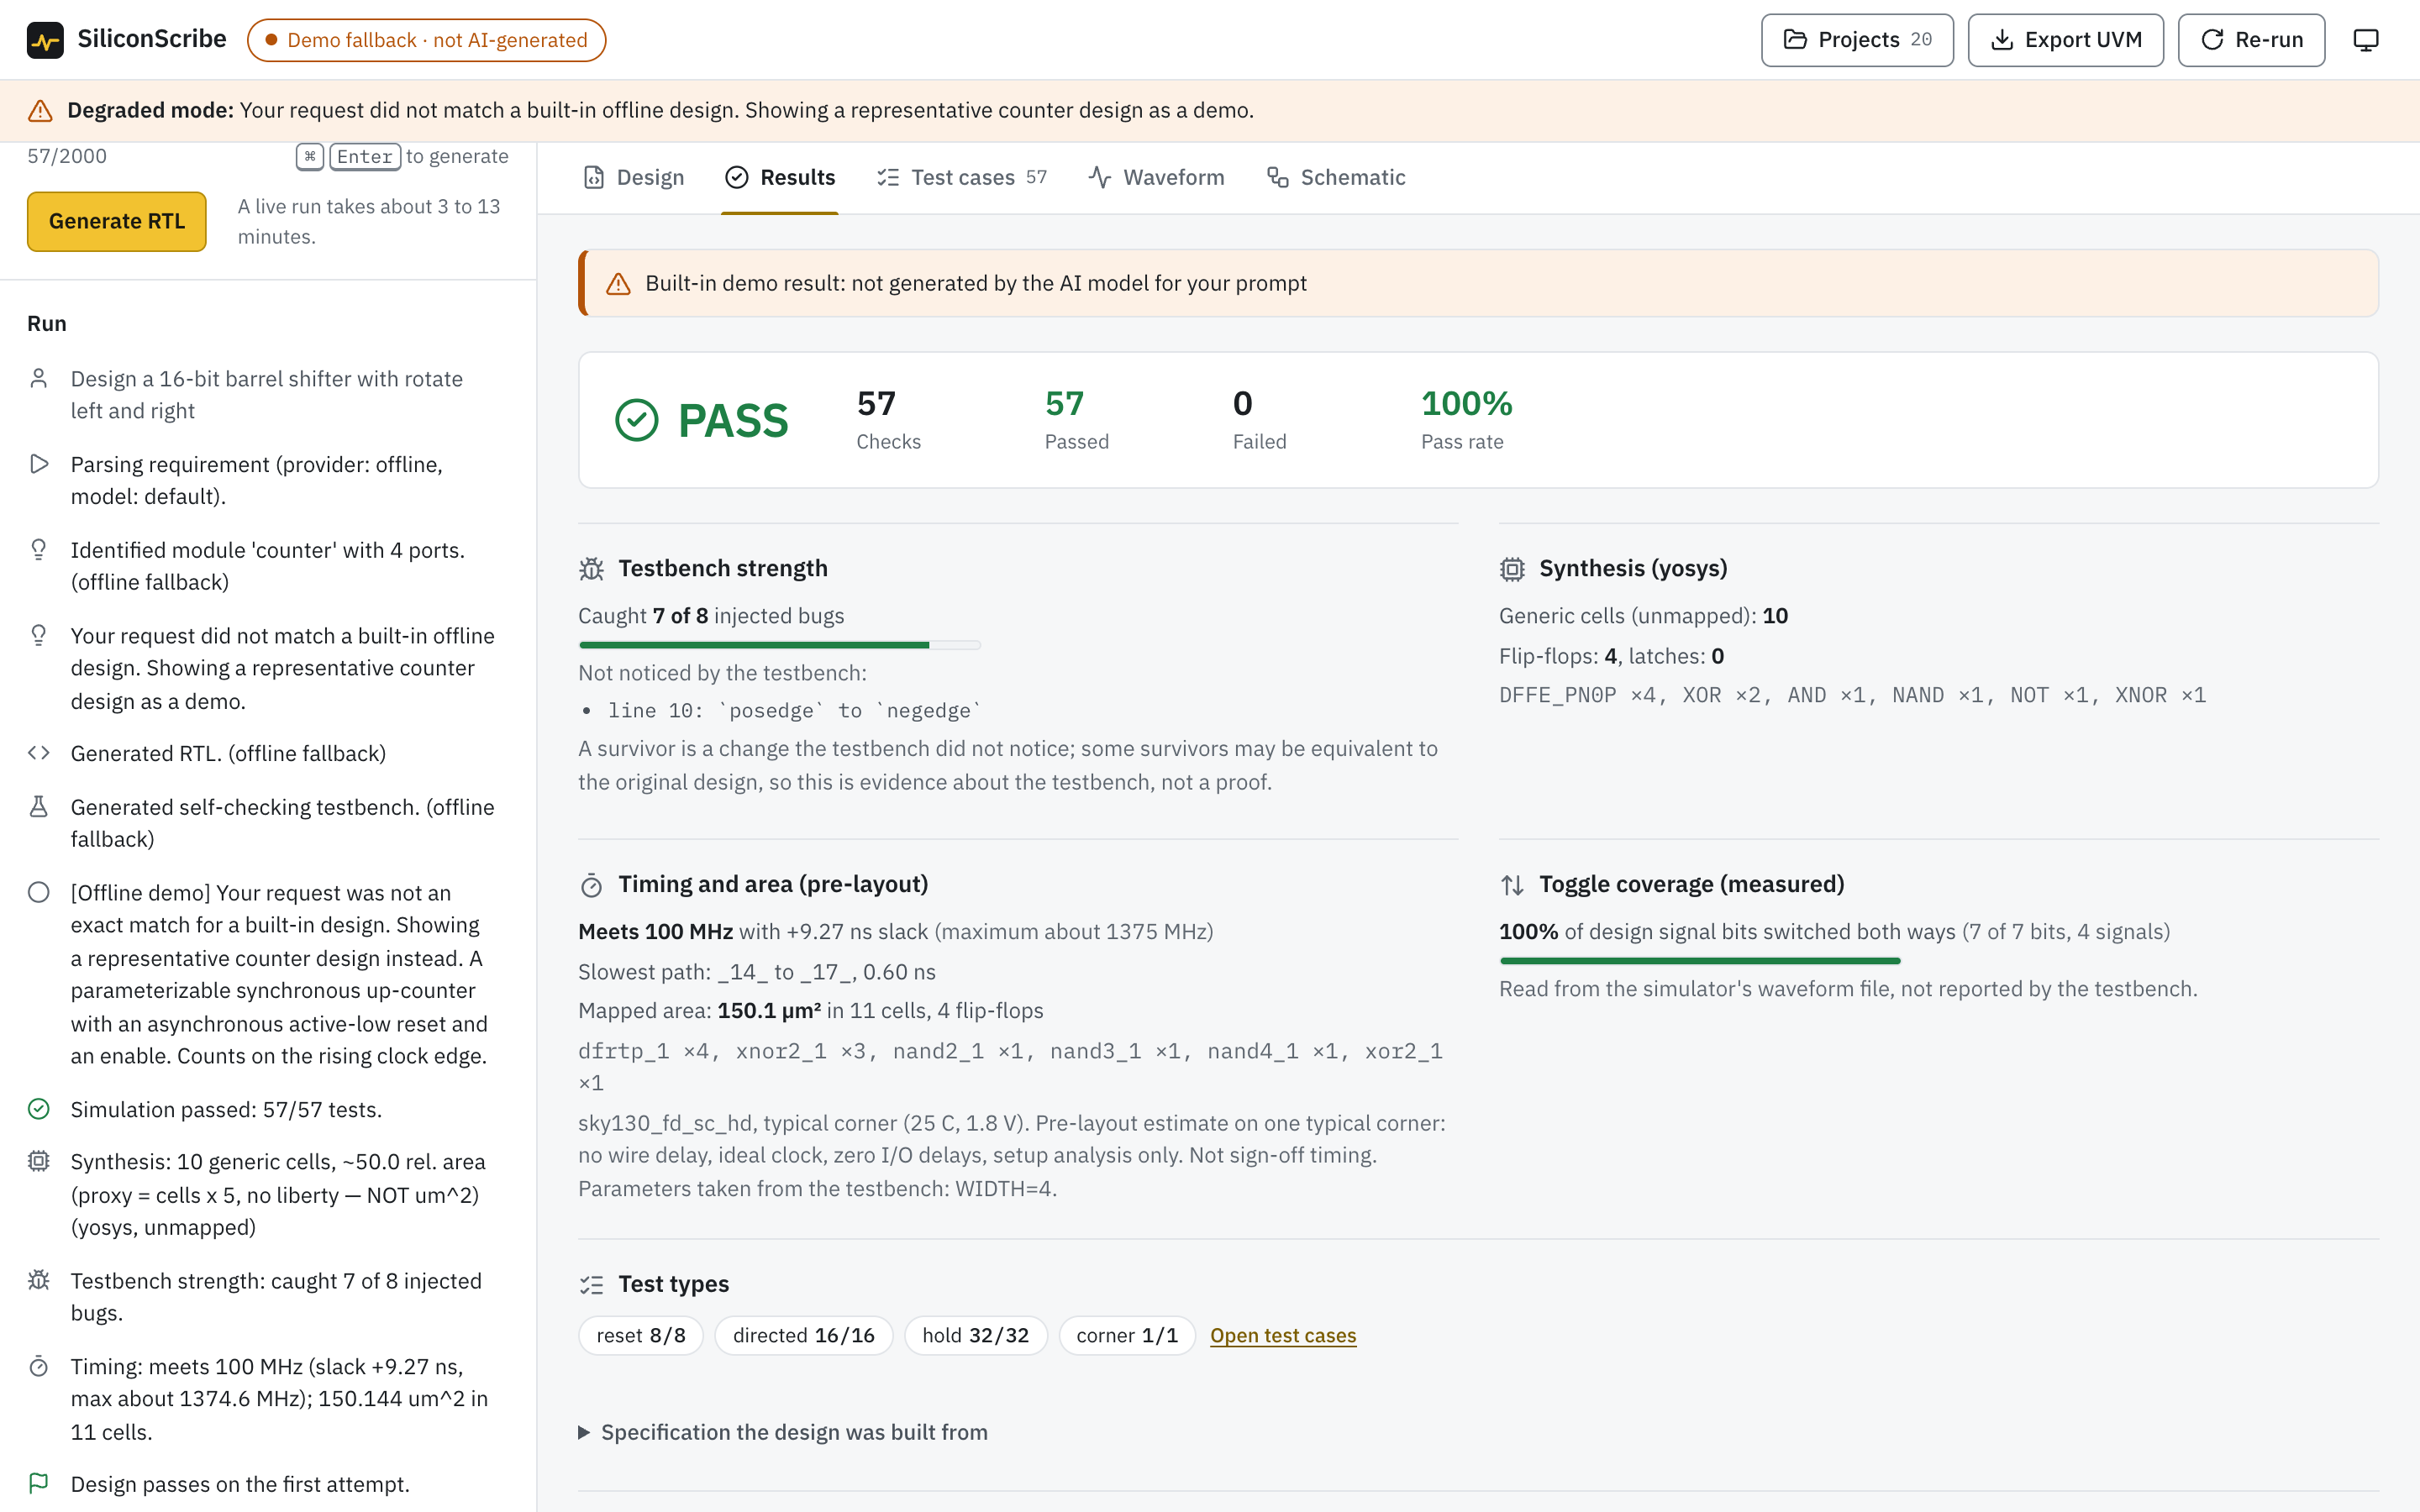
\includegraphics[width=0.65\textwidth]{s15_offline_demo.png}
\caption[Labelled fallback to the built-in demo]{A run that fell back to the built-in demo is labelled as such (degraded-mode banner and ``not generated by the AI model'' notice). The strength (7 of 8), timing (meets 100 MHz, 150.1\,\textmu m$^2$, 11 cells) and toggle-coverage sections describe the built-in counter that ran.}
\label{fig:degraded}
\end{figure}

\section{Final Security and Robustness Review}
\label{sec:review}
Before submission the system was probed the way an examiner or attacker might, using executable probes against the running API rather than code reading alone. Table~\ref{tab:review} lists the findings and their measured before/after behaviour. One suspected path was refuted: command execution through \code{$system()} does not work on Icarus Verilog 12.0, which reports the task as undefined; the sandbox policy still rejects it because other simulator builds define it.

\begin{table}[H]
\centering
\caption{Findings of the final review and their measured effect.}
\label{tab:review}
\footnotesize
\begin{tabularx}{\textwidth}{@{}p{3.1cm}p{3.7cm}p{3.2cm}X@{}}
\toprule
\textbf{Finding} & \textbf{Probe} & \textbf{Before} & \textbf{After} \\
\midrule
Testbench could read and write arbitrary files & planted secret file plus file-I/O tasks sent to the simulation endpoint & secret returned in the API response; file written outside the workspace & rejected by the sandbox policy; nothing leaked or written; 18 regression tests \\
One run froze the server & health check while an 8~s simulation runs & 6.5~s & 1~ms (blocking routes run in a thread pool; rate limiter locked) \\
Weak testbenches & 14-mutant sweep & 11 of 14 killed & 14 of 14 killed \\
Browser runs never saved & generate in the UI, open the drawer & not listed & listed; regression test \\
Tests wrote to the real database & row count before and after the suite & grew on every run & unchanged (isolated workspace) \\
Duplicated interface text & screenshots & bit range printed twice on waveform labels; degraded notice shown twice & each shown once \\
\bottomrule
\end{tabularx}
\end{table}

\subsection{Second review round}
\label{sec:review2}
After submission the whole system was reviewed again, this time by several independent reviewers (verification, security, backend design, interface and tests), and each claimed defect was reproduced before it was fixed. Table~\ref{tab:review2} lists what was found. Three results matter most for the question ``is a PASS trustworthy?'': the design under test could write its own verdict, the sandbox was a deny-list that could be sidestepped by task-name variants, and the repair loop could weaken the testbench that judges it.

\begin{table}[H]
\centering
\caption{Findings of the second review round (each reproduced, fixed and covered by a regression test).}
\label{tab:review2}
\footnotesize
\begin{tabularx}{\textwidth}{@{}p{3.2cm}p{4.0cm}p{3.0cm}X@{}}
\toprule
\textbf{Finding} & \textbf{Probe} & \textbf{Before} & \textbf{After} \\
\midrule
Forgeable verdict & wrong design whose own \code{initial} block prints \code{Passed: 200 / Failed: 0 / ALL TESTS PASSED}, optionally followed by \code{$finish} & reported PASS & design may not print the summary lines or end the run; summary must be whole lines, last pair wins; \code{FAIL}/\code{ERROR} lines contradict \code{Failed: 0}; zero checks is not a PASS \\
Sandbox deny-list gaps & file-access variants (\code{$fopena}, \code{$fputc}, \code{$ivlh_*}) & not on the deny-list & system tasks are allow-listed; anything else is rejected before compile \emph{and} before lint \\
Repair loop could weaken the oracle & fixer rewrites the testbench & accepted if it still printed PASS & minimum executed-check floor, design-instance check, original testbench re-run on the final design with an explicit warning if the oracle changed \\
Spoofable rate limit & 25 requests with a forged \code{X-Forwarded-For} & 25 of 25 accepted against 20 per minute & socket address used unless the deployment declares a trusted proxy \\
Resource limits & a testbench using about 1~GB for about 20~s & ran inside the old limits & CPU-time, file-size and memory limits plus at most two simulations at once (the memory limit is enforced on Linux, not macOS) \\
Re-run in the interface & edit the code and press Re-run & testbench checks skipped; previous waveform and warning left on screen & zero-check guard; waveform, repair timeline and warning refreshed; application-level regression test \\
Other correctness defects & a valid testbench with a one-second delay; port-width mismatches; multi-module replies; provider outages & false FAIL; hidden as warnings; truncated to the first module; recognised by digits in the message text & correct verdict; width mismatch is an error; all modules kept; typed upstream error \\
Weak curated testbenches & mutation sweep extended from 14 to 27 mutants & survivors found by the reviewers & 27 of 27 killed \\
Silently shortened test labels & a test type named \code{undefined_opcode} shown in the new Test cases tab & shown as \code{fined_opcode} (a Verilog string in a 12-character register keeps only its rightmost characters) & registers widened to 24 and 64 characters; a regression test runs a real simulation \\
\bottomrule
\end{tabularx}
\end{table}

The same review added a \emph{Test cases} tab to the results panel. It lists every executed check with its type (for example reset, directed, hold, exhaustive), its time, the expected and actual values and the result, with per-type pass ratios, filters, a bit-level difference for failures and a jump to that moment in the waveform. These rows are parsed from one \code{CHK|...} line per comparison; the verdict is decided by the validated summary, and since the fourth review round a \code{CHK|FAIL} row can only make it stricter (a FAIL), never turn it into a PASS. The waveform viewer was redesigned in the same round (signals grouped by role, value at the cursor, radix selection, two measurement cursors, flags at failed checks, fit-to-width zoom and a full-window mode).

\subsection{Third review round: timing stage and model access}
\label{sec:review3}
When the timing stage was added, it was attacked in the same way, by giving it designs chosen to break it. Table~\ref{tab:review3} lists what was found and fixed; its last two rows are defects of the later equivalence check, found when it was run on the evaluation designs, and each is now a regression test. The model menu was hardened at the same time: the API accepts browser calls from this machine only (extra exact origins are opt-in through \code{CORS_ALLOW_ORIGINS}), and every model id is validated before it can reach a subprocess or a URL (Section~\ref{sec:trustimpl}).

\begin{table}[H]
\centering
\caption{Defects found in the timing stage and its equivalence check, and their fixes.}
\label{tab:review3}
\footnotesize
\begin{tabularx}{\textwidth}{@{}p{4.0cm}p{4.6cm}X@{}}
\toprule
\textbf{Probe} & \textbf{Before} & \textbf{After} \\
\midrule
Design built from sub-modules & only the top module counted (area about 40\% too low); its clock was missed & hierarchy flattened before mapping \\
Clock not named \code{clk} & not recognised as a clock & clocks read from the mapped netlist; several clocks supported \\
Tri-state output & silently turned into a wire and reported as meeting 100 MHz & refused with a reason \\
Combinational loop & a meaningless maximum frequency & refused with a reason \\
Testbench overrides a parameter & a different circuit timed from the one simulated & numeric overrides applied before mapping \\
Equivalence check with \code{x} allowed on inputs & SAT ``disproved'' the correct ALU c7 with an input value containing \code{x} & inputs restricted to defined 0/1 values \\
Design built from an initialised array (c5) & equivalence check could not run (SAT cannot model memory initialisation) & RTL passed through Yosys \code{memory} first, as synthesis does \\
\bottomrule
\end{tabularx}
\end{table}

\subsection{Fourth review round: nine engineering roles}
\label{sec:review4}
Before the viva the whole tool (not the documents) was reviewed once more by nine reviewers, each taking one engineering role: ASIC design, design verification, backend systems, security, LLM integration, frontend, interface design, test engineering and release engineering. About 110 findings were reported; each was reproduced before it was fixed, every fix has a regression test, and each fix was checked by deliberately undoing it and confirming that a test fails. A tenth, independent reviewer then received only the findings and the change set, tried to break the fixes, and found a macro-argument sandbox bypass, a regular-expression slowdown introduced by the fixes and three regressions; those were fixed in the same way. All 123 saved runs and the 14 evaluation designs give the same verdicts with the old and the new code. Table~\ref{tab:review4} lists the findings that matter most.

\begin{table}[H]
\centering
\caption{Most important findings of the fourth review round (each reproduced, fixed and covered by a regression test).}
\label{tab:review4}
\footnotesize
\begin{tabularx}{\textwidth}{@{}p{4.2cm}p{4.4cm}X@{}}
\toprule
\textbf{Probe} & \textbf{Before} & \textbf{After} \\
\midrule
Testbench with a comment or a macro around \code{$dumpfile} / \code{$fopen} & wrote a file outside the workspace; run reported PASS & rules also applied after comment removal and to the macro-expanded source \\
Repair keeps the bug and edits the expected values & plain PASS, warnings only in text & shown as ``PASS, disputed''; the oracle may be rewritten only after a compile failure \\
Phase counters, \code{CHK|FAIL} rows, design forging the summary through \code{final} or \texttt{\%c} & PASS & FAIL, or refused before compiling \\
Port wider than 64 bits & upper bits never compared & check task widened to 256 bits; wider ports carry a warning \\
Slow one-check testbench in mutation testing & every timed-out mutant counted as caught (3 of 3) & timeouts of a slow testbench are inconclusive \\
64-bit register; slow path on a second clock & refused as ``no logic''; reported as meeting 500 MHz & timed correctly; misses timing \\
Flip-flop on the other clock edge; register with a declaration value & equivalence ``proven'' & ``not proven'' with the reason \\
Two runs of the same design at once & wrong verdict in 25 of 25 tries & one run per design folder at a time \\
Compile timeout & compiler child left at 100\% CPU & whole process group stopped; compile under CPU and memory limits \\
Quota error during a repair & whole run lost & run kept, with the reason \\
Partly unknown value shown in decimal & whole page blank & formatter never fails; error boundary around the results \\
Live run after the review: correct SR latch, testbench releases the forbidden input on both pins at once (zero-delay oscillation, simulated time stops) & TIMEOUT shown as ``0 checks, 0\%''; last output lost to \texttt{SIGKILL} & still TIMEOUT, but ``552 checks before stop'', no pass rate, and the likely cause named; \texttt{SIGTERM} first so the output is kept \\
\bottomrule
\end{tabularx}
\end{table}

\paragraph{What this does not establish.} The verdict is still only as strong as the testbench that prints it. Model-written testbenches are now measured on every PASS (strength, toggle coverage and, after a testbench-changing repair, a second opinion), but these measures are evidence, not proof: the strength score is a sample of up to 12 syntactic mutants and only toggle coverage is measured. The formal equivalence check covers only the step from RTL to netlist, not the RTL itself. The sandbox remains defence in depth on a developer machine, not a multi-tenant jail.
